\documentclass[a4paper, 11pt,reqno]{article}
\input{macro/package.tex}
\input{macro/environement}
% Header et footer

\pagestyle{fancy}
\fancyhead{}
\fancyfoot{}
\renewcommand{\headwidth}{\textwidth}
\renewcommand{\footrulewidth}{0.4pt}
\renewcommand{\headrulewidth}{0pt}
\renewcommand{\footruleskip}{5px}

\fancyfoot[R]{Olivier Glorieux}
%\fancyfoot[R]{Jules Glorieux}

\fancyfoot[C]{ Page \thepage }
\fancyfoot[L]{1BIOA - Lycée Chaptal}
%\fancyfoot[L]{MP*-Lycée Chaptal}
%\fancyfoot[L]{Famille Lapin}

\input{macro/newcommand.tex}
\geometry{hmargin=1.0cm, vmargin=2.5cm}


\newcommand{\type}{TD }
\excludecomment{correction}
%\newcommand{\type}{Correction TD }

\begin{document}
\title{TD 15 : Polynômes}


\section{\large{Op\'erations sur les polyn\^omes}}
%-----------------------------------------------
\begin{exercice}  \;
	On pose $P=X^2+3X$, $Q=X^2+X+1$, $S=X^2-1$.
	\begin{enumerate}
		\item Calculer $P^2$, $P-Q$ et $P^2-Q^2$.
		      %\item Calculer $P(Q)$, $Q(P)$ et $P(R)-R(P)$.
		\item Calculer $P(X+1)$.
		\item Calculer $S\circ f$ avec $f: t\mapsto \cos{(t)}$.
	\end{enumerate}
\end{exercice}

\begin{correction}  \;
	\begin{enumerate}
		\item Les calculs donnent $P^2=X^4+6X^3+9X^2$, $P-Q=2X-1$, $P^2-Q^2=4X^3+6X^2-2X-1$.
		      %\item Il s'agit ici de composer des polyn\^{o}mes. Les calculs donnent: $P(Q)=Q^2+3Q=X^4+2X^3+6X^2+5X+4$, $Q(P)=P^2+P+1=X^4+6X^3+10X^2+3X+1$ et $P(R)-R(P)=-9X^5-29X^4-24X^3+2X^2$.
		\item On obtient $P(X+1)=X^2+5X+4$.
		\item $S\circ f : t \mapsto -\sin^2(t) $.
	\end{enumerate}
\end{correction}



%-----------------------------------------------
\begin{exercice}
	D\'evelopper le polyn\^ome suivant: $Q=(X^3+X^2+X+1)\ddp \sum\limits_{k=0}^{2n} (-1)^kX^k.$
\end{exercice}

\begin{correction}
	On d\'eveloppe $Q=(X^3+X^2+X+1)\sum\limits_{k=0}^{2n} (-1)^kX^k$ et on obtient:\\
	\noindent $Q=\sum\limits_{k=0}^{2n} (-1)^kX^{k+3}+\sum\limits_{k=0}^{2n} (-1)^kX^{k+2}+\sum\limits_{k=0}^{2n} (-1)^kX^{k+1}+\sum\limits_{k=0}^{2n} (-1)^kX^{k}$. On fait alors des changements de variable dans les trois premi\`{e}res sommes et les indices de sommation \'etant muets, on obtient:\\
	\noindent $Q=-\sum\limits_{k=3}^{2n+3} (-1)^kX^k+\sum\limits_{k=2}^{2n+2} (-1)^kX^k-\sum\limits_{k=1}^{2n+1} (-1)^kX^k+\sum\limits_{k=0}^{2n} (-1)^kX^k.$ En utilisant alors la relation de Chasles, on obtient:
	$Q=X^{2n+3}+X^{2n+1}+X^2+1$. On a utilis\'e aussi le fait que: $(-1)^{2k-3}=(-1)^{2n+3}=(-1)^{2k-1}=(-1)^{2n+1}=(-1)^3=(-1)^1=-1$ et $(-1)^{2k-2}=(-1)^{2n+2}=(-1)^{2k}=(-1)^{2n}=(-1)^2=(-1)^0=1$.
\end{correction}




%-----------------------------------------------
\begin{exercice}  \;
	Simplifier le polyn\^ome $\ddp R=\sum\limits_{k=0}^n \ddp \binom{n}{k} 3^k(1-X)^{3n-2k}X^k$.
\end{exercice}
\begin{correction}  \;
	On cherche \`{a} faire appara\^{i}tre la formule du bin\^{o}me de Newton. On a:
	$$R=\sum\limits_{k=0}^n \ddp \binom{n}{k} 3^k(1-X)^{3n-2k}X^k=
		\sum\limits_{k=0}^n \ddp \binom{n}{k} (3X)^k\lbrack (1-X)^3\rbrack^{n-k}(1-X)^k$$
	car $\lbrack (1-X)^3\rbrack^{n-k}(1-X)^k= (1-X)^{3n-3k} (1-X)^k=(1-X)^{3n-2k}$. On obtient alors:
	$$R=\sum\limits_{k=0}^n \ddp \binom{n}{k} \lbrack3X(1-X)\rbrack^k\lbrack (1-X)^3\rbrack^{n-k}$$
	et sous cette forme on reconna\^{i}t la formule du bin\^{o}me de Newton. Ainsi on obtient: $R=\left(  3X(1-X)+(1-X)^3  \right)^n$, soit : \fbox{$R=(1-X)^n (X^2+X+1)^n$}.
\end{correction}




%-----------------------------------------------
\begin{exercice}
	Calculer $P(Q)$ et $Q(P)$ avec $P=X^2-3X+1$ et $Q=X^2-3X+2$.
\end{exercice}
\begin{correction}
	Les calculs donnent: $P(Q)=Q^2-3Q+1=X^4-6X^3+10X^2-3X-1$ et $Q(P)=P^2-3P+2=X^4-6X^3+8X^2+2X$.
\end{correction}

\section{\large{Degr\'e et coefficients}}

%-----------------------------------------------
\begin{exercice}  \;
	Dans les deux cas suivants, d\'eterminer tous les polyn\^omes $P$ v\'erifiant les conditions indiqu\'ees
	\begin{enumerate}
		\item $\mathrm{deg}(P)=3$ et $P(1)=4,\ P(-1)=0,\ P(-2)=-5,\ P(2)=15$.
		\item $\mathrm{deg}(P)\leq 2$ et $P^2=X^4+2X^3-3X^2-4X+4$.
	\end{enumerate}
\end{exercice}

\begin{correction}  \;
	\begin{enumerate}
		\item On sait donc que $P$ est de degr\'e 3 et que -1 est racine de $P$. Ainsi $P$ est de la forme $P=(X+1)(aX^2+bX+c)$. Puis on utilise le fait que: $P(1)=4$, $P(-2)=-5$ et $P(2)=15$. Ces trois conditions permettent d'obtenir le syst\`{e}me suivant: $\left\lbrace\begin{array}{lll}  a+b+c&=&2\vsec\\4a-2b+c&=&5\vsec\\4a+2b+c&=&5  \end{array}\right.$. La r\'esolution donne: $a=1$, $b=0$ et $c=1$. On a donc ainsi entierement d\'etermin\'e $P$: \fbox{$P=(X+1)(X^2+1)$}.
		      %----
		\item Comme $\deg{P}\leq 2$, on cherche $P$ sous la forme: $P=aX^2+bX+c$. Les calculs donnent: $P^2=a^2X^4+2ab X^3+(b^2+2ac)X^2+2bcX+c^2$. Puis par unicit\'e des coefficients d'un polyn\^{o}me, on doit r\'esoudre le syst\`{e}me suivant: $\left\lbrace\begin{array}{lll}  a^2&=&1\vsec\\ab&=&1 \vsec\\b^2+2ac&=&-3\vsec\\ bc&=& -2\vsec\\c^2&=&4  \end{array}\right.$. Comme $a^2=1$, on a: $a=-1$ ou $a=1$. De m\^{e}me comme $c^2=4$, on a: $c=-2$ ou $c=2$. \'Etudions les 4 possibilit\'es que l'on a:
		      \begin{itemize}
			      \item[$\bullet$] si $a=1$ et $c=2$: comme $ab=1$, on a: $b=1$. Mais comme $bc=-2$, $b=-1$: impossible.
			      \item[$\bullet$] si $a=-1$ et $c=-2$: comme $ab=1$, on a: $b=-1$. Mais comme $bc=-2$, $b=1$: impossible.
			      \item[$\bullet$] si $a=1$ et $c=-2$: comme $ab=1$, on a: $b=1$ et ainsi $bc=-2$. Et on a aussi alors $b^2+2ac=-3.$
			      \item[$\bullet$] si $a=-1$ et $c=2$: $b=-1$ v\'erifie bien $ab=1$, $bc=-2$ et $b^2+2ac=-3$.
		      \end{itemize}
		      Ainsi il y a deux solutions qui sont: \fbox{$P=-X^2-X+2$ et $P=X^2+X-2$}.
	\end{enumerate}
\end{correction}





%-----------------------------------------------
\begin{exercice}   \;
	D\'eterminer le degr\'e et le coefficient dominant des polyn\^omes suivants o\`u $n$ d\'esigne un entier strictement positif et $P$ un polyn\^ome de degr\'e $n$ et de coefficient dominant $a_n\not= 0$.
	\begin{enumerate}
		\begin{minipage}[t]{0.45\textwidth}
			\item $(X^4+1)^3$
			\item $(X+1)^n-(X-1)^n$
		\end{minipage}
		\quad
		\begin{minipage}[t]{0.45\textwidth}
			\item $P^2-P+1$
			\item $Q=P(X+1)-P$
			\item $\sum\limits_{k=0}^n P^{(k)}$.
		\end{minipage}
	\end{enumerate}
\end{exercice}

\begin{correction}  \;
	\begin{enumerate}
		\item On a: $(X^4+1)^3=P(Q)$ avec $P=X^3$ et $Q=X^4+1$. Ainsi par propri\'et\'e sur le degr\'e d'une compos\'ee de polyn\^{o}mes, on obtient que $\deg{(X^4+1)^3}=12$. De plus, en d\'eveloppant avec le bin\^{o}me de Newton, on obtient que le coefficient dominant est 1.
		      %----
		\item On pose $P=(X+1)^n-(X-1)^n=Q-R$. Par propri\'et\'e sur le degr\'e d'une somme de polyn\^{o}mes de m\^{e}me degr\'e, on sait que $\deg{P}\leq \deg{Q}$, \`{a} savoir: $\deg{P}\leq n$. Pour conna\^{i}tre exactement son degr\'e, il faut regarder les termes de plus haut degr\'e dans $Q$ et $R$ et regarder s'ils s'annulent. Par le bin\^{o}me de Newton, on sait que: $\ddp Q=\sum\limits_{k=0}^n \binom{n}{k} X^k$ et $R=\ddp \sum\limits_{k=0}^n \binom{n}{k} (-1)^{n-k} X^k$. On commence par regarder les termes en $X^n$ et on obtient: $\ddp P=\binom{n}{n} X^n-\binom{n}{n}(-1)^0 X^n+T$ avec $T\in\R_{n-1}\lbrack X\rbrack$. Ainsi les termes devant $X^n$ s'annulent et donc $\deg{P}\leq n-1$. On regarde donc maintenant les termes devant $X^{n-1}$ et on obtient $\ddp P=\binom{n}{n-1} X^{n-1}-\binom{n}{n-1}(-1)^1 X^{n-1}+T=2nX^{n-1}+T$ avec $T\in\R_{n-2}\lbrack X\rbrack$. Comme $2n\not= 0$, on vient de d\'emontrer que \fbox{$\deg{P}=n-1$ et son coefficient dominant est $2n$}.
		      %----
		\item Par propri\'et\'e sur le degr\'e d'une compos\'ee, on sait que $\deg{P^2}=2n$ et par propri\'et\'e sur le degr\'e d'une somme, on a: $\deg{(P+1)}\leq n$. Comme $2n\not= n$ car $n\in\N^{\star}$, par propri\'et\'e sur le degr\'e d'une somme de polyn\^{o}mes de degr\'e diff\'erents, on obtient que: \fbox{$\deg{(P^2+P+1)}=2n$}. Et si $a_n$ est le coefficient dominant de $P$, alors \fbox{$a_n^2$ est le coefficient dominant de $P^2+P+1$} car $a_n^2$ est le coefficient dominant de $P^2$.
		      %----
		\item Par propri\'et\'e sur le degr\'e d'une compos\'ee de polyn\^{o}mes, on sait que $\deg{P(X+1)}=\deg{P}$. Puis par propri\'et\'e sur le degr\'e d'une somme de polyn\^{o}mes de m\^{e}me degr\'e, on obtient que: $\deg{Q}\leq \deg{P}$. \'Etudions les termes en $X^n$ pour savoir s'ils s'annulent ou pas. On a: $P=a_nX^n+T$ avec $T\in\R_{n-1}\lbrack X\rbrack$. Ainsi, on obtient que: $Q=a_n(X+1)^n +T(X+1)-a_nX^n-T=a_n X^n-a_n X^n +R$ avec $R\in\R_{n-1}\lbrack X\rbrack$ en utilisant le bin\^{o}me de Newton afin de d\'evelopper le terme en $(X+1)^n$. Ainsi, on obtient que $Q=R$ et ainsi $\deg{Q}\leq n-1$. Il faut donc alors regarder les termes en $X^{n-1}$. Toujours en utilisant le bin\^{o}me de Newton et le fait que $P=a_nX^n+a_{n-1}X^{n-1}+T$ avec $T\in\R_{n-2}\lbrack X\rbrack$, on obtient que: $Q=a_n(X+1)^n+a_{n-1}(X+1)^{n-1}+T(X+1)-a_n X^n-a_{n-1}X^{n-1}-T=a_n\binom{n}{n-1}X^{n-1}+a_{n-1}X^{n-1}+T(X+1)-a_{n-1}X^{n-1}-T=na_nX^{n-1}+R$ avec $R\in\R_{n-2}\lbrack X\rbrack$. Comme $a_n\not= 0$ et $n\in\N^{\star}$, on a que: \fbox{$na_n\not= 0$ et ainsi $\deg{ Q}=n-1$ de coefficient dominant $na_n$}.
		\item Par propri\'et\'e sur le degr\'e d'une d\'eriv\'ee, on sait que: $\deg{ P^{(k)}}=\deg{P}-k$ si $k\leq \deg{P}$ ce qui est le cas car la somme va de $k=0$ \`{a} $k=n=\deg{P}$. Ainsi, on doit trouver le degr\'e d'une somme de polyn\^{o}mes de degr\'e tous diff\'erents, et par propri\'et\'e, on sait alors que le degr\'e correspond au maximum et ainsi on a: $\deg{\left( \sum\limits_{k=0}^n P^{(k)}\right)}=\deg{P^{(0)}}=\deg{P}=n$. Et le coefficient dominant correspond donc au coefficient dominant de $P^{(0)}=P$, \`{a} savoir $a_n$.
	\end{enumerate}
\end{correction}







%-----------------------------------------------
\begin{exercice}  \;
	Soient les polyn\^omes $P=X^2-X+1\; \hbox{et}\; Q=X^3-X.$
	Pour tout entier $n\geq 1$, on d\'efinit par r\'ecurrence les polyn\^omes $P_n$ par
	$$\left\lbrace\begin{array}{l}
			P_1=P\vsec \\
			P_{n+1}=XP_n(Q)+2QP_n.
		\end{array}\right.$$
	\begin{enumerate}
		\item Calculer $P_2$.
		\item Calculer les degr\'es de $P_2$ et de $P_3$.
		\item D\'eterminer pour tout entier $n\in\N$ le degr\'e de $P_n$.
		\item D\'eterminer le coefficient dominant de $P_n$.
	\end{enumerate}
\end{exercice}
\begin{correction}  \;
	\begin{enumerate}
		\item Les calculs donnent: $P_2=XP(Q)+2Q\times P=X^7-5X^4+3X^3+3X^2-X$.
		\item On a donc $\deg{P_2}=7$ et en utilisant les propri\'et\'es sur le degr\'e d'un produit et d'une compos\'ee de polyn\^omes, on obtient : $\deg{P_3}=22$.
		\item
		      \begin{itemize}
			      \item[$\bullet$] Comme on n'arrive pas \`{a} conjecturer directement l'expression du degr\'e de $P_n$, on va obtenir une relation de r\'ecurrence en utilisant la relation de r\'ecurrence qui d\'efinit la suite des polyn\^{o}mes. On note $d_n=\deg{P_n}$. On sait que: $P_{n+1}=XP_n(Q)+2QP_n$. Par propri\'et\'e sur le degr\'e d'un produit de polyn\^{o}mes, on sait que:
			            $\deg{QP_n}=3+d_n$. De m\^{e}me, par propri\'et\'e sur le degr\'e d'une compos\'ee et d'un produit de polyn\^{o}mes, on obtient que: $\deg{XP_n(Q)}=3d_n+1$. Comme $3d_n+1> 3+d_n$ d\`{e}s que $d_n>1$ ce qui est toujours le cas (car les degr\'es sont de plus en plus grands et le degr\'e de $P_1$ est $2$), on a par propri\'et\'e sur le degr\'e d'une somme de polyn\^{o}mes dont les degr\'es sont diff\'erents: $\deg{P_{n+1}}=3d_n+1$, \`{a} savoir: $d_{n+1}=3d_n+1$.
			      \item[$\bullet$] On reconna\^{i}t donc une suite arithm\'etico-g\'eom\'etrique de premier terme $d_1=2$ et dont la relation de r\'ecurrence est: $d_{n+1}=3d_n+1$. Les calculs donnent que pour tout $n\in\N$: \fbox{$d_n=7\times 3^{n-1}-\ddp\demi$}.
		      \end{itemize}
		\item Les calculs faits pour $P_2$ et $P_3$ permettent de conjecturer que le coefficient dominant est 1. On le montre par r\'ecurrence en utilisant la relation de r\'ecurrence qui d\'efinit la suite des polyn\^{o}mes. A faire.
	\end{enumerate}
\end{correction}




%-----------------------------------------------
\begin{exercice}  \;
	\noindent On d\'efinit une suite de polyn\^omes $(P_n)_{n\in\N}$ par :$\ddp \left\lbrace\begin{array}{l} P_0=1,\ P_1=X\vsec \\
			\forall n\in\N,\ P_{n+2}=XP_{n+1}+\left( 1-\ddp\frac{X^2}{4}\right)P_n.
		\end{array}\right.$
	\begin{enumerate}
		\item Calculer $P_2$ et $P_3$.
		\item D\'emontrer que, pour tout $n\in\N$, $P_n$ est de degr\'e inf\'erieur ou \'egal \`a $n$.
		\item Pour tout $n\in\N$, on note $a_n$ le coefficient d'indice $n$ de $P_n$.
		      \begin{enumerate}
			      \item Donner les valeurs de $a_0,\ a_1,\ a_2$ et $a_3$.
			      \item Montrer que : $\forall n\in\N,\ a_{n+2}=a_{n+1}-\ddp\frac{a_n}{4}.$\\
			            En d\'eduire une expression de $a_n$ en fonction de $n$ pour tout $n\in\N$ puis le degr\'e du polyn\^ome $P_n$.
		      \end{enumerate}
	\end{enumerate}
\end{exercice}
\begin{correction}  \;
	\begin{enumerate}
		\item On obtient $P_2=\ddp \frac{3}{4} X^2 +1$ et $P_3=\ddp \frac{1}{2} X^3 + 2X$.
		\item Montrons par r\?ecurrence double la propri\'et\'e $H_n : \deg(P_n)\leq n$.
		      \begin{itemize}
			      \item[$\bullet$] Initialisation : On a $\deg(P_0)=0\leq 0$ et et $\deg(P_1)=1\leq 1$, donc $H_0$ et $H_1$ sont vraies.
			      \item[$\bullet$] H\'er\'edit\'e : Soit $n \in \N$ fix\'e, on suppose $H_n$ et $H_{n+1}$ vraies, montrons que $H_{n+2}$ est vraie.\\
			            D'apr\`es  $H_n$ et $H_{n+1}$, et peut \'ecrire $P_n= a_n X^n + R$ et $P_{n+1}=a_{n+1} X^{n+1} + S$ avec $R\in \R_{n-1}[X]$ et $S \in \R_{n}[X]$. Donc on obtient, par d\'efinition de la suite :
			            $$\begin{array}{rcl}
					            P_{n+2} & = & \ddp X(a_{n+1} X^{n+1} + S) + \left(1-\frac{X^2}{4} (a_{n} X^{n}+R\right)\vsec      \\
					                    & = & \ddp \left(a_{n+1} - \frac{a_n}{4} \right) X^{n+2} + XS +a_n X^n - \frac{X^2 R}{2}.
				            \end{array}$$
			            Or par somme et produit de polyn\^omes, on a $\deg(XS)\leq 1+n=n+1$, $\deg(a_n X^n)=n$ et $\deg(X^2R)\leq 2+n-1=n+1$. Donc finalement le degr\'e de $P_{n+2}$ est inf\'erieur ou \'egal \`a $n+2$, et le coefficient de $X^{n+2}$ vaut $a_{n+2} = a_{n+1} - \ddp \frac{a_n}{4}$ (ce coefficient pourrait s'annuler).
		      \end{itemize}
		      Par principe de r\'ecurrence, on a donc \fbox{$\deg(P_n)\leq n$}.
		\item
		      \begin{enumerate}
			      \item D'apr\`es les calculs pr\'ec\'edents, on a \fbox{$a_0=1, a_1=1, a_2 = \ddp \frac{3}{4}, a_3= \frac{1}{2}$}.
			      \item D'apr\`es la question 2), on a bien $a_{n+2} = a_{n+1} - \ddp \frac{a_n}{4}$.\\
			            On en d\'eduit que $(a_n)_{n\in \N}$ est une suite r\'ecurrente lin\'eaire double. On calcule alors son terme g\'en\'eral gr\^ace \`a la m\'ethode vue en cours, et on obtient \fbox{$a_n=(1+n) \ddp \frac{1}{2^n}$}. On en d\'eduit que le coefficient d'indice $n$ est non nul, donc \fbox{$P_n$ est bien de degr\'e $n$}.
		      \end{enumerate}
	\end{enumerate}
\end{correction}
%-----------------------------------------------

%-----------------------------------------------
\begin{exercice}  \;
	Soit $n\in\N^{\star}$.
	\begin{enumerate}
		\item Exprimer de deux fa\c{c}ons diff\'erentes le coefficient de $X^n$ dans le polyn\^ome: $P=(1+X)^n(1+X)^n.$
		\item En d\'eduire l'expression de $\ddp \sum\limits_{k=0}^n \binom{n}{k}^2$.
	\end{enumerate}
\end{exercice}
\begin{correction}  \;
	\begin{enumerate}
		\item
		      \begin{itemize}
			      \item[$\bullet$] On peut par exemple remarquer que $P=(X+1)^{2n}$ et on peut alors utiliser le bin\^{o}me de Newton qui nous donne: $P=\ddp\sum\limits_{k=0}^{2n} \binom{2n}{k} X^k$. Ainsi le coefficient devant $X^n$ vaut $\binom{2n}{n}$.
			      \item[$\bullet$] Mais on peut aussi voir $P$ comme le produit $(X+1)^n\times (X+1)^n$ et en utilisant encore le bin\^{o}me de Newton, on obtient:
			            $$\begin{array}{rcl}
					            P & = & \ddp\sum\limits_{k=0}^{n} \binom{n}{k} X^k\times \sum\limits_{j=0}^{n} \binom{n}{j} X^j \vsec                                                                            \\
					              & = & \ddp \left( \binom{n}{0} X^0 + \binom{n}{1} X^1 + \ldots + \binom{n}{n}X^n \right) \times \left( \binom{n}{0} X^0 + \binom{n}{1} X^1 + \ldots + \binom{n}{n}X^n \right).
				            \end{array}$$
			            On cherche alors \`{a} d\'evelopper ces deux sommes et \`{a} regarder quels sont les termes qui vont faire appara\^{i}tre du $X^n$ : le $X^0$ de la premi\`{e}re somme doit \^{e}tre multipli\'e avec du $X^n$ de la deuxi\`{e}me somme, le $X$ de la premi\`{e}re somme avec du $X^{n-1}$ de la deuxi\`{e}me somme, \dots, le $X^{n-1}$ de la premi\`{e}re somme avec le $X$ de la deuxi\`{e}me somme et enfin le $X^n$ de la premi\`{e}re somme avec le $X^0$ de la deuxi\`{e}me somme. Donc pour tout $k\in\intent{ 0,n}$, le $X^k$ de la premi\`{e}re somme doit \^{e}tre
			            multipli\'e avec le $X^{n-k}$ de la de la deuxi\`{e}me somme.
			            Ainsi, cela nous donne: $\ddp\sum\limits_{k=0}^n \binom{n}{k}\binom{n}{n-k}$ qui est le terme qui appara\^{i}t devant $X^n$.
		      \end{itemize}
		      Par unicit\'e des coefficients d'un polyn\^{o}me, on obtient que: $\ddp\sum\limits_{k=0}^n \binom{n}{k}\binom{n}{n-k}=\binom{2n}{n}$.
		\item Comme, par sym\'etrie des coefficients binomiaux, on sait que $\ddp\binom{n}{k}=\binom{n}{n-k}$, la formule pr\'ec\'edente devient: $\ddp\sum\limits_{k=0}^n \binom{n}{k}^2=\binom{2n}{n}$.
	\end{enumerate}
\end{correction}






\begin{exercice}
	Montrer que la d\'eriv\'ee n-i\`eme de la fonction $\tan{}$ est de la forme $P_n\circ \tan{}$ o\`u $P_n$ est un polyn\^ome de degr\'e $n+1$ dont on d\'eterminera le coefficient dominant.
\end{exercice}
\begin{correction}
	\'Etude de d\'eriv\'ees n-i\`eme:
	\begin{enumerate}
		\item La fonction $f$ est de classe $C^{\infty}$ sur $I=\rbrack -\ddp\frac{\pi}{2},\ddp\frac{\pi}{2}\lbrack$ comme quotient dont le d\'enominateur
		      ne s'annule pas de fonction $C^{\infty}$. De plus, le calcul donne
		      $$\forall x\in I,\quad f^{\prime}(x)=\ddp\frac{\sin{x}}{\cos^2{x}}\qquad \hbox{et}\qquad f^{(2)}(x)=
			      \ddp\frac{\cos^3{(x)} +2\sin^2{(x)}\cos{(x)}  }{\cos^4{(x)}}=\ddp\frac{1+\sin^2{(x)}}{\cos^3{(x)}}$$
		      en divisant tout par $\cos{x}$ qui pouvait \^etre mis en facteur au num\'erateur et en utilisant le fait que: $\cos^2{(x)}=1-\sin^2{(x)}$.
		\item
		      \begin{itemize}
			      \item[$\bullet$] On montre par r\'ecurrence sur $n\in\N$ la propri\'et\'e
			            $$\mathcal{P}(n):\quad f\ \hbox{est de classe}\ C^n\ \hbox{sur}\ I\ \hbox{et}\ \exists P_n\ \hbox{polyn\^ome tel que}\ \forall x\in I,\quad f^{(n)}(x)=\ddp\frac{P_n(\sin{x})}{(\cos{x})^{n+1}}.          $$
			      \item[$\bullet$] Initialisation: pour $n=0$:\\
			            \noindent La fonction $f$ est bien continue sur $\R$ comme quotient dont le d\'enominateur ne s'annule pas.\\
			            \noindent D'un c\^ot\'e, on a: $f^{(0)}(x)=\ddp\frac{1}{\cos{(x)}}$ et de l'autre c\^ot\'e, on a: $\ddp\frac{P_0(x)}{\cos{x}}$. Ainsi, si on pose $P_0=1$, ce polyn\^ome convient et $\mathcal{P}(0)$ est vraie.
			      \item[$\bullet$] H\'er\'edit\'e: soit $n\in\N$ fix\'e. On suppose la propri\'et\'e vraie au rang $n$, montrons qu'elle est vraie au rang $n+1$. Par hypoth\`ese de r\'ecurrence, on sait que la fonction $f$ est de classe $C^n$ sur $I$ et qu'il existe un polyn\^ome $P_n$ tel que
			            $$\forall x\in I,\quad f^{(n)}(x)=\ddp\frac{P_n(\sin{x})}{(\cos{(x)})^{n+1}}.$$
			            \begin{itemize}
				            \item[$\star$] Cette fonction $f^{(n)}$ est bien d\'erivable sur $I$ comme quotient dont le d\'enominateur ne s'annule pas.
				            \item[$\star$]
				                  On d\'erive $f^{(n)}$ et on obtient pour tout $x\in I$:
				                  $$\begin{array}{lll}
						                  f^{(n+1)}(x) & = & \ddp\frac{ P_n^{\prime}(\sin{x})\cos{x}\times\cos^{n+1}{x}-(n+1)P_n(\sin{x})\cos^n{(x)}(-\sin{x})       }{ \cos^{2n+2}{x} }\vsec \\
						                               & = & \ddp\frac{\cos^n{x}\left( P_n^{\prime}(\sin{x})\cos^2{(x)}+(n+1)P_n(\sin{x})\sin{x}         \right)}{\cos^{2n+2}{(x)}}\vsec      \\
						                               & = & \ddp\frac{   P_n^{\prime}(\sin{x})(1-\sin^2{x})+(n+1)P_n(\sin{x})\sin{x}     }{\cos^{n+2}{x}}.
					                  \end{array}$$
				                  Ainsi, si on pose
				                  $$P_{n+1}=(1-X^2)P_n^{\prime}+(n+1)XP_n,$$
				                  $P_{n+1}$ est bien un polyn\^ome comme somme de polyn\^omes.
				            \item[$\star$] Cette fonction $f^{(n+1)}$ est bien continue sur $I$ et donc $f$ est bien de classe $C^{n+1}$ sur $I$.
			            \end{itemize}
			            Ainsi $\mathcal{P}(n+1)$ est vraie.
			      \item[$\bullet$] Conclusion: il r\'esulte du principe de r\'ecurrence que pour tout $n\in\N$, il existe un polyn\^ome $P_n$ tel que
			            $$\forall x\in I,\quad f^{(n)}(x)=\ddp\frac{P_n(x)}{(\cos{x})^{n+1}}.$$
		      \end{itemize}
		\item Degr\'e et coefficient dominant de $P_n$:
		      \begin{itemize}
			      \item[$\bullet$] Le calcul des premiers polyn\^{o}mes de la suite donne: $P_0=1$, $P_1=X$, $P_2=X^2+1$, $P_3=X^3+5X$.
			      \item[$\bullet$] Ainsi on peut conjecturer que $\deg{P_n}=n$ et $a_n=1$ avec $a_n$ coefficient dominant de $P_n$.
			            \begin{itemize}
				            \item[$\star$] On montre par r\'ecurrence sur $n\in\N$ la propri\'et\'e $\mathcal{P}(n):\ \deg{P_n}=n,\ a_n=1$.
				            \item[$\star$] Initialisation: pour $n=0$: on a vu que $P_0=1$ donc on a: $\deg{P_0}=0$ et $a_0=1$. Donc $\mathcal{P}(0)$ est vraie.
				            \item[$\star$] H\'er\'edit\'e: soit $n\in\N$ fix\'e, on suppose vraie la propri\'et\'e \`{a} l'ordre $n$, montrons qu'elle est vraie \`{a} l'ordre $n+1$. Par hypoth\`{e}se de r\'ecurrence, on sait que: $P_n=X^n+T$ avec $T\in\R_{n-1}\lbrack X\rbrack$. De plus, on sait que $P_{n+1}=(1-X^2)P_n^{\prime}+(n+1)XP_n$ donc on obtient que: $P_{n+1}=(1+X^2)(nX^{n-1}+T^{\prime})+(n+1)X ( X^{n}+T)=X^{n+1}+R$ avec $R=n X^{n-1}+(1-X^2)T^{\prime}+(n+1)XT$. Et $R\in \R_{n}\lbrack X\rbrack$ par propri\'et\'e sur le degr\'e d'une d\'eriv\'ee, d'un produit et d'une somme de polyn\^{o}mes. Ainsi on a bien que: $\deg{P_{n+1}}=n+1$ et $a_{n+1}=1$. Donc $\mathcal{P}(n+1)$ est vraie.
				            \item[$\star$] Conclusion: il r\'esulte du principe de r\'ecurrence que pour tout $n\in\N$: $\deg{P_n}=n$ et le coefficient dominant de $P_n$ est $1$.
			            \end{itemize}
		      \end{itemize}
	\end{enumerate}
\end{correction}


%%-----------------------------------------------
\begin{exercice}
	Montrer que la d\'eriv\'ee n-i\`eme de la fonction $x\mapsto \ddp\frac{1}{1+x^2}$ est de la forme
	$$x\mapsto \ddp\frac{P_n(x)}{(1+x^2)^{n+1}}$$
	o\`u $P_n$ esst un polyn\^ome de degr\'e $n$ dont on d\'eterminera le coefficient dominant.
\end{exercice}

\begin{correction}
	\begin{enumerate}
		\item On sait donc que $P$ est de degr\'e 3 et que -1 est racine de $P$. Ainsi $P$ est de la forme $P=(X+1)(aX^2+bX+c)$. Puis on utilise le fait que: $P(1)=4$, $P(-2)=-5$ et $P(2)=15$. Ces trois conditions permettent d'obtenir le syst\`{e}me suivant: $\left\lbrace\begin{array}{lll}  a+b+c&=&2\vsec\\4a-2b+c&=&5\vsec\\4a+2b+c&=&5  \end{array}\right.$. La r\'esolution donne: $a=1$, $b=0$ et $c=1$. On a donc ainsi entierement d\'etermin\'e $P$: $P=(X+1)(X^2+1)$.
		\item Comme $\deg{P}\leq 2$, on cherche $P$ sous la forme: $P=aX^2+bX+c$. Les calculs donnent: $P^2=a^2X^4+2ab X^3+(b^2+2ac)X^2+2bcX+c^2$. Puis par unicit\'e des coefficients d'un polyn\^{o}me, on doit r\'esoudre le syst\`{e}me suivant: $\left\lbrace\begin{array}{lll}  a^2&=&1\vsec\\ab&=&1 \vsec\\b^2+2ac&=&-3\vsec\\ bc&=& -2\vsec\\c^2&=&4  \end{array}\right.$. Comme $a^2=1$, on a: $a=-1$ ou $a=1$. De m\^{e}me comme $c^2=4$, on a: $c=-2$ ou $c=2$. \'Etudions les 4 possibilit\'es que l'on a:
		      \begin{itemize}
			      \item[$\bullet$] si $a=1$ et $c=2$: comme $ab=1$, on a: $b=1$. Mais comme $bc=-2$, $b=-1$: impossible.
			      \item[$\bullet$] si $a=-1$ et $c=-2$: comme $ab=1$, on a: $b=-1$. Mais comme $bc=-2$, $b=1$: impossible.
			      \item[$\bullet$] si $a=1$ et $c=-2$: comme $ab=1$, on a: $b=1$ et ainsi $bc=-2$. Et on a aussi alors $b^2+2ac=-3.$
			      \item[$\bullet$] si $a=-1$ et $c=2$: $b=-1$ v\'erifie bien $ab=1$, $bc=-2$ et $b^2+2ac=-3$.
		      \end{itemize}
		      Ainsi il y a une deux solutions qui sont: $P=-X^2-X+2$ et $P=X^2+X-2$.
	\end{enumerate}
\end{correction}


%-----------------------------------------------
\begin{exercice}
	Soit la fonction $f$ d\'efinie sur $\rbrack -\ddp\frac{\pi}{2},\ddp\frac{\pi}{2}\lbrack$ par: $f(x)=\ddp\frac{1}{\cos{x}}$.
	\begin{enumerate}
		\item Calculer $f^{\prime}$ et $f^{\prime\prime}$.
		\item Montrer par r\'ecurrence l'existence, pour tout $n\in\N$, d'un polyn\^ome $P_n$ tel que, pour tout $x\in\rbrack -\ddp\frac{\pi}{2},\ddp\frac{\pi}{2}\lbrack$:
		      $$f^{(n)}(x)=\ddp\frac{P_n(\sin{x})}{(\cos{x})^{n+1}}.$$
		      Trouver une relation entre $P_{n+1}$, $P_n$ et $P^{\prime}_n$.
		\item D\'eterminer le mon\^ome de plus haut degr\'e de $P_n$.
	\end{enumerate}
\end{exercice}


\begin{correction}
	\begin{enumerate}
		\item Voir la fiche sur les polyn\^{o}mes. Cela permet de montrer que pour tout $n\in\N$: $\deg{P_n}=n$ et son coefficient dominant est $(-2)^n$.
		\item
		      \begin{itemize}
			      \item[$\bullet$] Calcul de $P_2=4X^2-2$ et $P_3=-8X^3+12X$.
			      \item[$\bullet$] On note par exemple $b_n$ le coefficient constant du polyn\^{o}me $P_n$. On peut conjecturer que $b_{2n+1}=0$, par contre, on ne trouve pas de relation simple pour $b_{2n}$. On va donc faire une identification des coefficients constants dans la relation de r\'ecurrence afin de trouver une relation de r\'ecurrence entre $b_{2n+2}$ et $b_{2n}$. On a: $P_{2n+2}=XQ_2+b_{2n+2}$ avec $Q_2\in\R_{2n+1}\lbrack X\rbrack$, $P_{2n+1}=XQ_1+b_{2n+1}$ avec $Q_1\in\R_{2n}\lbrack X\rbrack$ et $P_{2n}=XQ+b_{2n}$ avec $Q\in\R_{2n-1}\lbrack X\rbrack$. En rempla\c{c}ant dans la relation de r\'ecurrence, on obtient: $XQ_2+b_{2n+2}=-2X(XQ_1+b_{2n+1})-2(2n+1)(XQ+b_{2n})=XR-2(2n+1)b_{2n}$ avec $R=-2X(XQ_1+b_{2n+1})-2(2n+1)XQ$. Ainsi par unicit\'e des coefficients d'un polyn\^{o}me, on a: $b_{2n+2}=-2(2n+1)b_{2n}$.
			      \item[$\bullet$] Si on it\`{e}re la relation de r\'ecurrence: $b_{2n+2}=-2(2n+1)b_{2n}$ valable pour tout $n\in\N$, on obtient:
			            $$\begin{array}{lll} b_{2n} & = & -2(2n-1)b_{2n-2}=(-2)^2 (2n-1)(2n-3)b_{2n-4}=(-2)^3 (2n-1)(2n-3)(2n-5)b_{2n-6}=\dots\vsec \\
                          & = & (-2)^n (2n-1)(2n-3)(2n-5)\dots \times 3\times 1  \times b_0.\end{array}$$
			            On a ainsi conjecturer la valeur du terme constant. Avant de faire la r\'ecurrence permettant de d\'emontrer cette relation, simplifions cette \'egalit\'e:
			            $$\begin{array}{lll} b_{2n} & = & (-1)^n 2^n \ddp\frac{ (2n)\times (2n-1)\times (2n-2)\times (2n-3)\times (2n-4)\dots 4\times 3\times 2\times 1  }{ (2n)\times (2n-2)\times (2n-4)\dots 4\times 2   }\vsec \\
                          & = & (-1)^n 2^n \ddp\frac{(2n)!}{ 2^n( n\times (n-1)\times (n-2)\times\dots \times 2\times 1  )  }=\ddp\frac{(-1)^n\times (2n)!}{n!}\end{array}$$
			      \item[$\bullet$]
			            \begin{itemize}
				            \item[$\star$] On montre par r\'ecurrence sur $n\in\N$ la propri\'et\'e: $\mathcal{P}(n):\ b_{2n}=\ddp\frac{(-1)^n\times (2n)!}{n!} \ \mathrm{et}\ b_{2n+1}=0$.
				            \item[$\star$] Initialisation: pour $n=0$, on a d'un c\^{o}t\'e: $b_{2\times 0}=b_0=1$ car $P_0=1$ et de l'autre c\^{o}t\'e:
				                  $\ddp\frac{(-1)^0 (0)!}{0!}=1$. De plus, on a aussi d'un c\^{o}t\'e: $b_{2\times 0+1}=b_1=0$ car $P_1=-2X$ et de l'autre c\^{o}t\'e: 0. Donc $\mathcal{P}(0)$ est vraie.
				            \item[$\star$] H\'er\'edit\'e: soit $n\in\N$ fix\'e, on suppose que $\mathcal{P}(n)$ est vraie, montrons que $\mathcal{P}(n+1)$ est vraie. Par hypoth\`{e}se de r\'ecurrence, on suppose donc que $b_{2n}=\ddp\frac{(-1)^n\times (2n)!}{n!} $ et $b_{2n+1}=0$. On cherche \`{a} montrer que $b_{2n+2}=\ddp\frac{(-1)^{n+1}\times (2n+2)!}{(n+1)!} $ et $b_{2n+3}=0$. D'apr\`{e}s la relation de r\'ecurrence qui d\'efinit la suite des polyn\^{o}mes, on a: $P_{2n+2}=-2XP_{2n+1}-2(2n+1)P_{2n}$.  On a: $P_{2n+2}=XQ_2+b_{2n+2}$ avec $Q_2\in\R_{2n+1}\lbrack X\rbrack$, $P_{2n+1}=XQ_1+b_{2n+1}$ avec $Q_1\in\R_{2n}\lbrack X\rbrack$ et $P_{2n}=XQ+b_{2n}$ avec $Q\in\R_{2n-1}\lbrack X\rbrack$. En rempla\c{c}ant dans la relation de r\'ecurrence, on obtient: $XQ_2+b_{2n+2}=-2X(XQ_1+b_{2n+1})-2(2n+1)(XQ+b_{2n})=XR-2(2n+1)b_{2n}$ avec $R=-2X(XQ_1+b_{2n+1})-2(2n+1)XQ$. Ainsi par unicit\'e des coefficients d'un polyn\^{o}me, on a:
				                  $b_{2n+2}=-2(2n+1)b_{2n}=-2(2n+1)\ddp\frac{(-1)^n\times (2n)!}{n!} $ par hypoth\`{e}se de r\'ecurrence. Ainsi, on a: $b_{2n+2}=(-1)^{n+1}  \ddp\frac{2\times (2n+2)(2n+1)(2n)!}{(2n+2)n!}=(-1)^{n+1}\ddp\frac{(2n+2)!}{(n+1)n!}=\ddp\frac{(-1)^{n+1}\times (2n+2)!}{(n+1)!} $.
				                  D'apr\`{e}s la relation de r\'ecurrence qui d\'efinit la suite des polyn\^{o}mes, on a aussi: $P_{2n+3}=-2XP_{2n+2}-2(2n+2)P_{2n+1}$.  On a: $P_{2n+3}=XQ_3+b_{2n+3}$ avec $Q_3\in\R_{2n+2}\lbrack X\rbrack$, $P_{2n+2}=XQ_2+b_{2n+2}$ avec $Q_2\in\R_{2n+1}\lbrack X\rbrack$ et $P_{2n+1}=XQ_1+b_{2n+1}$ avec $Q_1\in\R_{2n}\lbrack X\rbrack$. En rempla\c{c}ant dans la relation de r\'ecurrence, on obtient: $XQ_3+b_{2n+3}=-2X(XQ_2+b_{2n+2})-2(2n+2)(XQ_1+b_{2n+1})=XR-2(2n+2)b_{2n+1}$ avec $R=-2X(XQ_2+b_{2n+2})-2(2n+2)XQ_1$. Ainsi par unicit\'e des coefficients d'un polyn\^{o}me, on a: $b_{2n+3}=-2(n+1)b_{2n+1}=0.$ Donc $\mathcal{P}(n+1)$ est vraie.
				            \item[$\star$] Conclusion: il r\'esulte du principe de r\'ecurrence que pour tout $n\in\N$: $b_{2n+1}=0$ et $b_{2n}=\ddp\frac{(-1)^n\times (2n)!}{n!}$.
			            \end{itemize}
		      \end{itemize}
		\item On peut remarquer sur $P_0$, $P_2$ et $P_4$ ne poss\`{e}dent que des puissances paires et sont donc des fonctions paires tandis que $P_1$, $P_3$ ne poss\`{e}dent que des puissances impaires et sont donc des fonctions impaires. On peut donc conjecturer que $P_{2n}$ est une fonction paire tandis que $P_{2n+1}$ est une fonction impaire.
		      \begin{itemize}
			      \item[$\bullet$] On montre par r\'ecurrence sur $n\in\N$ la propri\'et\'e $\mathcal{P}(n):\ P_{2n}\ \mathrm{est\ une\ fonction\ paire\ et}\ P_{2n+1}\ \mathrm{est\ une\ fonction\ impaire}$.
			      \item[$\bullet$] Initialisation: pour $n=0$: on sait que $P_0=1$ et donc $P_0$ est bien une fonction paire. De m\^{e}me, on sait que $P_1=-2X$ et ainsi $P_1$ est bien une fonction impaire.
			      \item[$\bullet$] H\'er\'edit\'e: soit $n\in\N$ fix\'e, on suppose que $\mathcal{P}(n)$ est vraie, montrons que $\mathcal{P}(n+1)$ est vraie. On commence par montrer que $P_{2n+2}$ est bien une fonction paire: on sait que $P_{2n+2}=-2XP_{2n+1}-2(2n+1)P_{2n}$. Comme par hypoth\`{e}se de r\'ecurrence, on sait que $P_{2n}$ est une fonction paire, $P_{2n}$ n'a donc que des puissances paires. De m\^{e}me, comme par hypoth\`{e}se de r\'ecurrence, on sait que $P_{2n+1}$ est une fonction impaire, $P_{2n+1}$ n'a donc que des puissances impaires et ainsi $-2XP_{2n+1}$ est un polyn\^{o}me n'ayant que des puissances paires. Donc par somme $P_{2n+2}$ n'a que des puissances paires et ainsi c'est une fonction paire. On montre alors que $P_{2n+3}$ est bien une fonction impaire: on sait que $P_{2n+3}=-2XP_{2n+2}-2(2n+2)P_{2n+1}$. Comme par hypoth\`{e}se de r\'ecurrence, on sait que $P_{2n+1}$ est une fonction impaire, $P_{2n+1}$ n'a donc que des puissances impaires. De plus, on vient de montrer que $P_{2n+2}$ est une fonction paire, $P_{2n+2}$ n'a donc que des puissances paires et ainsi $-2XP_{2n+2}$ est un polyn\^{o}me n'ayant que des puissances impaires. Donc par somme $P_{2n+3}$ n'a que des puissances impaires et ainsi c'est une fonction impaire. Donc $\mathcal{P}(n+1)$ est vraie.
			      \item[$\bullet$] Conclusion: il r\'esulte du principe de r\'ecurrence que pour tout $n\in\N$, $P_{2n}$ est une fonction paire et $P_{2n+1}$ est une fonction impaire.
		      \end{itemize}
	\end{enumerate}
\end{correction}




%-----------------------------------------------
\begin{exercice}
	Soit la fonction $f:\ \rbrack -1,1\lbrack\rightarrow\R$ d\'efinie pour tout $x$ r\'eel par
	$$f(x)=\ddp\frac{1}{\sqrt{1-x^2}}.$$
	\begin{enumerate}
		\item Calculer $f^{\prime}$ et $f^{\prime\prime}$.
		\item Montrer par r\'ecurrence que la d\'eriv\'ee n-i\`eme est de la forme
		      $$f^{(n)}(x)=\ddp\frac{P_n(x)}{(1-x^2)^n\ \sqrt{1-x^2}}$$
		      o\`u $P_n$ est un polyn\^ome.\\
		      \noindent Donner une relation $(R)$ entre $P_{n+1}$, $P_n$ et $P_n^{\prime}$.
		\item Montrer que $P_n$ est une fonction paire si $n$ est un entier pair et une fonction impaire si $n$ est un entier impaire.
		\item Montrer par r\'ecurrence en utilisant la relation $(R)$ que
		      $$P_n^{\prime}=n^2P_{n-1}.$$
		\item En d\'eduire que les polyn\^omes $P_n$ v\'erifient pour tout entier $n\geq 1$ la relation de r\'ecurrence suivante
		      $$P_{n+1}=(2n+1)XP_n+n^2(1-X^2)P_{n-1}.$$
	\end{enumerate}
\end{exercice}

\begin{correction}
	.......
\end{correction}
%-----------------------------------------------




%-------------------------------------------------
%------------------------------------------------
%\vspace{0.5cm}
%\noindent\section{\large{D\'erivation et formule de Taylor-Lagrange}}
%
%%-----------------------------------------------
\begin{exercice}
	Soit $n\in\N^{\star}$. Calculer la d\'eriv\'ee $n$-i\`eme du polyn\^ome suivant:
	$$P=X^2(1+X)^n.$$
\end{exercice}

\begin{correction}
	Calculons la d\'eriv\'ee $n$-i\`eme du polyn\^ome suivant: $P=X^2(1+X)^n.$
	\begin{itemize}
		\item[$\bullet$] Le polyn\^{o}me $P$ s'\'ecrit comme le produit de deux polyn\^{o}mes: $P=QR$ avec $Q=X^2$ et $R=(1+X)^n$. Pour calculer la d\'eriv\'ee $n$-i\`{e}me de ce polyn\^{o}me, on va donc utiliser la formule de Leibniz. On a alors:
		      $P^{(n)}=\sum\limits_{k=0}^n \binom{n}{k} Q^{(k)} R^{(n-k)}$.
		\item[$\bullet$] Calcul de $Q^{(k)}$: comme $Q$ est un polyn\^{o}me de degr\'e 2, on a: si $k>2$ alors $Q^{(k)}=0$. Sinon: $Q^{(0)}=Q$, $Q^{\prime}=2X$ et $Q^{(2)}=2$.
		\item[$\bullet$] Calcul de $R^{(n-k)}$: On a: $R^{(n-k)}=\ddp\frac{n!}{k!}(1+X)^k$ si $k\geq 0$ ce qui est toujours le cas car dans la formule de Leibniz on somme pour $k$ allant de 0 \`{a} $n$.
		\item[$\bullet$] On obtient: $P^{(n)}=\sum\limits_{k=0}^2 \binom{n}{k} Q^{(k)} R^{(n-k)}+\sum\limits_{k=3}^n \binom{n}{k} Q^{(k)} R^{(n-k)}$ par Chasles. Puis:
		      $$ \begin{array}{lll}P^{(n)}&=&\sum\limits_{k=0}^2 \binom{n}{k} Q^{(k)} R^{(n-k)}=QR^{(n)}+nQ^{\prime}R^{(n-1)}+\ddp\frac{n(n-1)}{2} Q^{(2)}R^{(n-2)}\vsec\\ &=& n!X^2+2nn!X(1+X)+n!\ddp\frac{n(n+1)}{2}(1+X)^2.\end{array}$$
	\end{itemize}
\end{correction}



%%-----------------------------------------------
\begin{exercice}
	Soit $n$ un entier non nul. On note alors $P$ le polyn\^ome: $P=X^n(1-X)^n$.
	\begin{enumerate}
		\item Calculer $P^{(n)}$.
		\item En d\'eduire que: $\sum\limits_{k=0}^n (-1)^{n-k}\binom{n}{k}^2= \ddp\frac{2^n}{n!}P^{(n)}\left( \ddp\demi \right) $.
		\item Montrer que: $P=\left( \ddp\frac{1}{4}-\left(X-\ddp\demi\right)^2  \right)^n$.
		\item En d\'eduire une expression de $P$ comme combinaison lin\'eaire des polyn\^omes
		      $$1,\left(X-\ddp\demi\right),\left(X-\ddp\demi\right)^2,\left(X-\ddp\demi\right)^3,\dots,\left(X-\ddp\demi\right)^{2n}.$$
		\item En d\'eduire la valeur de: $\sum\limits_{k=0}^n (-1)^{n-k} \binom{n}{k}^2$.
	\end{enumerate}
\end{exercice}
%-----------------------------------------------
\begin{exercice}
	Soit le polyn\^ome $P=X^5-X^4+3X^2+X-5$.\\
	\noindent D\'eterminer les coefficients du polyn\^ome $P(X+1)$ avec un minimum de calcul.
\end{exercice}
\begin{correction}
	Voir??
\end{correction}
%-----------------------------------------------

%-------------------------------------------------
%------------------------------------------------
\vspace{0.2cm}
% 
%-------------------------------------------------
%------------------------------------------------
\noindent\section{\large{Racines d'un polyn\^{o}me}}

%-----------------------------------------------
\begin{exercice}  \;
	Trouver toutes les racines de $P=X^4-5X^3+7X^2-5X+6$ dans $\bC$.
\end{exercice}
\begin{correction}  \;
	On peut remarquer que $i$ est racine de $P$ et comme $P\in\R$, on sait donc que $-i$ aussi est racine de $P$. On peut tout de suite remarquer que $i$ n'est pas racine de $P^{\prime}$ et donc $i$ et $-i$ sont racines simples de $P$. On peut aussi remarquer que 2 est racine de $P$ et que $P^{\prime}(2)\not= 0$. Ainsi 2 est aussi racine simple de $P$.
	Ainsi on peut factoriser $P$ par $(X+i)(X-i)(X-2)=(X^2+1)(X-2)$. L'identification des polyn\^{o}mes donne que 3 est racine de $P$ et que $P$ se factorise dans $\bC$ sous la forme: \fbox{$P=(X-i)(X+i)(X-2)(X-3)$}. On est s\^{u}r d'avoir bien trouv\'e toutes les racines car on a 4 racines et $P$ est un polyn\^{o}me de degr\'e 4.\\
	Remarque : on peut \'egalement trouver la derni\`ere racine en utilisant : $i \times (-i) \times 2 \times x_4 = (-1)^4 \ddp\frac{6}{1}$, donc $x_4 = 3$.
\end{correction}





%-----------------------------------------------
\begin{exercice}  \;
	Soit $n\in\N^{\star}$. On consid\`ere les polyn\^omes $A=(X+1)^n-(X-1)^n\; \hbox{et}\;B=\left(\ddp\sum\limits_{k=0}^n X^k\right)^2.$
	\begin{enumerate}
		\item Calculer le degr\'e de ces deux polyn\^omes.
		\item  D\'eterminer les racines de ces deux polyn\^omes.
	\end{enumerate}
\end{exercice}

\begin{correction}  \;
	\begin{enumerate}
		\item
		      \begin{enumerate}
			      \item Dans l'exercice ??? on a d\'ej\`{a} montr\'e que: $\deg{A}=n-1$.
			      \item On a: $B=P^2$ avec $P=\sum\limits_{k=0}^n X^k$. On a donc : $\deg{B}=2\deg{P}$. De plus, $\deg{P}=n$ donc $\deg{B}=2n$.
		      \end{enumerate}
		\item
		      \begin{enumerate}
			      \item
			            L'id\'ee ici est de se ramener \`{a} la r\'esolution d'une \'equation type racine n-i\`{e}me de l'unit\'e. On a d\'ej\`{a} par d\'efinition d'une racine d'un polyn\^{o}me que: $z$ est racine de $A$ si et seulement si $A(z)=0$ si et seulement si $(z+1)^n=(z-1)^n$.
			            \begin{itemize}
				            \item[$\bullet$] Comme 1 n'est pas solution de l'\'equation, on peut supposer que $z\not= 1$. Ainsi, on peut bien diviser par $(z-1)^n$ qui est bien non nul. Ainsi, on a
				                  $$(z+1)^n=(z-1)^n\Leftrightarrow \left( \ddp\frac{z+1}{z-1}\right)^n=1\Leftrightarrow Z^n=1$$
				                  en posant $Z=\ddp\frac{z+1}{z-1}$.
				            \item[$\bullet$] R\'esolution des racines n-i\`{e}mes de l'unit\'e (\`a savoir faire, cours) : on obtient apr\`es calculs que les solutions sont les $Z$ de la forme $\ddp Z_k=e^{\frac{2ik\pi}{n}},\quad k\in\intent{ 0,n-1}.$
				            \item[$\bullet$] On repasse alors \`{a} $z$ et on cherche donc les $z$ tels que: $\ddp\frac{z+1}{z-1}=e^{\frac{2ik\pi}{n}}$ avec $k\in\intent{ 0,n-1}$ fix\'e. On obtient alors
				                  $$\ddp\frac{z+1}{z-1}=e^{\frac{2ik\pi}{n}}\Leftrightarrow z+1=e^{\frac{2ik\pi}{n}} (z-1)\Leftrightarrow z\left(1- e^{\frac{2ik\pi}{n}} \right)=-e^{\frac{2ik\pi}{n}}-1\Leftrightarrow z\left(e^{\frac{2ik\pi}{n}} -1\right)=\left( e^{\frac{2ik\pi}{n}}+1\right).$$
				                  Ici, il faut faire attention car on ne peut JAMAIS diviser par un nombre sans v\'erifier qu'il est bien NON nul. Or on a:
				                  $$e^{\frac{2ik\pi}{n}} -1=0\Leftrightarrow e^{\frac{2ik\pi}{n}} =1\Leftrightarrow \ddp\frac{2k\pi}{n}=2k^{\prime}\pi\Leftrightarrow k=nk^{\prime}$$
				                  avec $k^{\prime}\in\Z$. Or $k\in\intent{ 0,n-1}$ donc le seul $k$ qui v\'erifie cela est $k=0$.
				                  \begin{itemize}
					                  \item[$\star$] Pour $k=0$, on obtient: $0=2$ donc il n'y a pas de solution pour $k=0$.
					                  \item[$\star$] Pour $k\not= 0$, \`{a} savoir pour $k\in\intent{ 1,n-1}$, on sait que $1- e^{\frac{2ik\pi}{n}}\not= 0$ et on peut donc bien diviser. On obtient
					                        $$z=\ddp\frac{e^{\frac{2ik\pi}{n}}+1}{e^{\frac{2ik\pi}{n}} -1}=-icot{\left( \ddp\frac{k\pi}{n} \right)}$$
					                        en utilisant la m\'ethode de l'angle moiti\'e.
				                  \end{itemize}
				            \item[$\bullet$] Les racines de $A$ sont donc $z=-i\cot{\left( \ddp\frac{k\pi}{n} \right)} $ avec $k\in\intent{ 1,n-1}$. On les bien toutes trouv\'ees puisque l'on en a $n-1$ et que le polyn\^{o}me est de degr\'e $n-1$.
			            \end{itemize}
			      \item On a: $z$ est racine de $B$ si et seulement si $B(z)=0$ si et seulement si $\sum\limits_{k=0}^n z^k=0$. Or on reconna\^{i}t une somme g\'eom\'etrique et ainsi, on a si $z\not= 1$: $\sum\limits_{k=0}^n z^k=\ddp\frac{1-z^{n+1}}{1-z}$. On remarque aussi que 1 n'est pas racine car $\sum\limits_{k=0}^n 1^k=n+1\not= 0$. Donc on peut bien supposer $z\not=1$. Ainsi, on a: $z$ est racine de $B$ si et seulement si: $\ddp\frac{1-z^{n+1}}{1-z}=0\Leftrightarrow z^{n+1}=1$. On reconna\^{i}t la r\'esolution des racines $n+1$-i\`{e}me de l'unit\'e. Les calculs donnent: $z_k=e^{\frac{2ik\pi}{n+1}}$ avec $k\in\intent{ 0,n}$. Mais comme $z\not= 1$, on doit enlever le cas $k=0$ qui donne 1. Ainsi les racines de $B$ sont les complexes de la forme:
			            $z_k=e^{\frac{2ik\pi}{n+1}}$ avec $k\in\intent{ 1,n}$. Et on a bien trouv\'e toutes les racines puisque l'on en a $n$ et que le degr\'e de $P$ est $n$.
		      \end{enumerate}
	\end{enumerate}
\end{correction}








%-----------------------------------------------
\begin{exercice}  \;
	Soit $n$ un entier non nul. Montrer que $a$ donn\'e est racine du polyn\^ome et d\'eterminer l'ordre de multiplicit\'e de cette racine
	\begin{enumerate}
		\item $a=2$ et $P=X^5-5X^4+7X^3-2X^2+4X-8$
		\item $a=1$ et $P=X^{2n}-nX^{n+1}+nX^{n-1}-1  $
		      %\item $a=1$ et $P=X^{2n}-n^2X^{n+1}+2(n^2-1)X^n-n^2X^{n-1}+1$
	\end{enumerate}
\end{exercice}
\begin{correction}  \;
	On regarde si $a$ est racine de $P$ et ainsi $a$ est au moins racine simple. Puis on regarde jusqu'\`{a} quelle d\'eriv\'ee de $P$, $a$ est-elle encore racine, ce qui donne l'ordre de multiplicit\'e de la racine $a$.
	\begin{enumerate}
		\item Les calculs donnent que: $P(2)=0=P^{\prime}(2)=P^{(2)}(2)$ et $P^{(3)}(2)\not= 0$. Ainsi $2$ est racine triple de $P$.
		\item Les calculs donnent que: $P(1)=0=P^{\prime}(1)=P^{(2)}(1)$ et $P^{(3)}(1)\not= 0$. Ainsi $1$ est racine triple de $P$.
		      %\item Les calculs donnent que: $P(1)=0=P^{\prime}(1)$ et $P^{(2)}(1)\not= 0$. Ainsi $1$ est racine double de $P$.
	\end{enumerate}
\end{correction}



%-----------------------------------------------
\begin{exercice}  \;
	D\'eterminer le nombre $a$ de mani\`ere  \`a ce que le polyn\^ome $P=X^5-aX^2-aX+1$ ait $-1$ comme racine au moins double.
\end{exercice}
\begin{correction}  \;
	Pour que $-1$ soit racine au moins double de $P$, on doit avoir: $P(-1)=0=P^{\prime}(-1)$. Les calculs donnent que: $P(-1)=-1-a+a+1=0$ donc $-1$ est racine au moins simple de $P$ sans condition sur $a$. On a de plus: $P^{\prime}=5X^4-2aX-a$. Ainsi, on obtient: $P^{\prime}(-1)=0\Leftrightarrow a=-5$. \\
	Donc \fbox{$-1$ racine au moins double de $P$ si et seulement si $a=-5$}.
\end{correction}
%------------------------------------------------
\begin{exercice}
	Soient $n\in\N^{\star}$ et les polyn\^omes
	$$P=1+X+\ddp\frac{X(X+1)}{2!}+\dots+\ddp\frac{X(X+1)\dots (X+n-1)}{n!}\ \hbox{et}\ Q=\ddp\frac{(X+n)(X+n-1)(X+n-2)\dots(X+1)}{n!}.$$
	\begin{enumerate}
		\item Calculer les degr\'es de $P$ et de $Q$ ainsi que $P(0)$ et $Q(0)$.
		\item Montrer que, pour tout $i\in\intent{ 1,n}$, on a: $Q(i)=\ddp \binom{n+i}{i}$.
		\item Montrer que, pour tout $i\in\intent{ 1,n}$, on a: $P(i)=\sum\limits_{k=0}^n \ddp \binom{i+k-1}{k}$.
		\item En d\'eduire que pour tout $i\in\intent{ 0,n}$, on a: $Q(i)=P(i)$
		\item En d\'eduire que $P=Q$.
	\end{enumerate}
\end{exercice}
\begin{correction}
	\begin{enumerate}
		\item
		      \begin{itemize}
			      \item[$\bullet$] On a: $P_n^{\prime}=\sum\limits_{k=1}^n \ddp\frac{k X^{k-1}}{k!}=\sum\limits_{k=1}^n \ddp\frac{X^{k-1}}{(k-1)!}=\sum\limits_{k=0}^{n-1} \ddp\frac{ X^{k}}{k!}=P_{n-1}$ en faisant le changement de variable $j=k-1$. Ainsi, on a, en utilisant la relation de Chasles: $P_n-P_n^{\prime}=P_n-P_{n-1}=\ddp\frac{X^n}{n!}$.
			      \item[$\bullet$] On suppose par l'absurde que $P_n$ admet une racine multiple que l'on note $\alpha$. Ainsi $\alpha$ est au moins racine double et ainsi on doit avoir \`{a} la fois $P_n(\alpha)=0$ et $P_n^{\prime}(\alpha)=0$. Ainsi, on a en particulier que: $P_n(\alpha)-P_{n}^{\prime}(\alpha)=0\Leftrightarrow \ddp\frac{\alpha^n}{n!}=0\Leftrightarrow \alpha=0$. Ainsi, si $\alpha$ est racine multiple de $P_n$ alors forc\'ement $\alpha=0$. Or on remarque que: $P_n(0)=1\not= 0$. Ainsi $0$ n'est pas racine de $P_n$. Contradiction. Donc $P_n$ n'admet pas de racine multiple.
		      \end{itemize}
		\item A NE PAS FAIRE.
		\item On a d\'ej\`{a} montr\'e que: $P_n^{\prime}=P_{n-1}$.
		\item
		      \begin{itemize}
			      \item[$\bullet$] On montre par r\'ecurrence sur $n\in\N$ la propri\'et\'e $\mathcal{P}(n):\ P_{2n}\ \mathrm{est\ une\ fonction\ strictement\ positive\ sur}\ \R\ \mathrm{et}\ P_{2n+1}$ s'annule une seule fois sur $\R$ en un r\'eel $\alpha_n<0$ en \'etant n\'egative avant et positive apr\`{e}s.
			      \item[$\bullet$] Initialisation: pour $n=0$:
			            \begin{itemize}
				            \item[$\star$] $P_0=1$ et donc $P_0$ est bien strictement positive sur $\R$.
				            \item[$\star$] $P_1=X+1$ et donc $P_1$ s'annule en $\alpha_1=-1<0$ et $P_1$ est bien n\'egative avant et positive apr\`{e}s.
			            \end{itemize}
			            Donc $\mathcal{P}(0)$ est vraie.
			      \item[$\bullet$] H\'er\'edit\'e: soit $n\in\N$ fix\'e, on suppose la propri\'et\'e vraie \`{a} l'ordre $n$, montrons qu'elle est vraie \`{a} l'ordre $n+1$.
			            \begin{itemize}
				            \item[$\star$] \'Etude de $P_{2n+2}$: on sait que $P_{2n+2}^{\prime}=P_{2n+1}$ et on conna\^{i}t par hypoth\`{e}se de r\'ecurrence le signe de $P_{2n+1}$. On obtient ainsi le tableau de variation de $P_{2n+2}$ suivant:
				                  \begin{center}
					                  \begin{tikzpicture}
						                  \sgnvar{ $x$          /,%
							                  $P_{2n+1}$       /,
							                  $P_{2n+2}$           /}%
						                  { $-\infty$,$\alpha_{n}$,$+\infty$}%
						                  \signe{ ,$-$,0,$+$, }
						                  \variation{
							                  +/$+\infty$            /,
							                  -/$P_{2n+2}(\alpha_n)$          /,%
							                  +/$+\infty$           /,%
						                  }
						                  %\valeur[draw]{1}{3}{1}{}{}   
						                  %\tkzTabTan[pos=below]{1}{3}{2}{$0$}                   
					                  \end{tikzpicture}
				                  \end{center}
				                  Les limites en $\pm\infty$ sont obtenues par le th\'eor\`{e}me du mon\^{o}me de plus haut degr\'e. De plus:
				                  $P_{2n+2}(\alpha_n)=\ddp\frac{\alpha_n^{2n+2}}{(2n+2)!}+P_{2n+1}(\alpha_n)=\ddp\frac{\alpha_n^{2n+2}}{(2n+2)!}$ par hypoth\`{e}se de r\'ecurrence. Et ainsi $P_{2n+2}(\alpha_n)>0$ et comme  $P_{2n+2}(\alpha_n)$ est le minimum global de $P_{2n+2}$, on a bien obtenu que $P_{2n+2}$ est strictement positive sur $\R$.
				            \item[$\star$] \'Etude de $P_{2n+3}$: on sait que $P_{2n+3}^{\prime}=P_{2n+2}$ et on vient de d\'emontrer que $P_{2n+2}$ reste toujours strictement positive sur $\R$. Ainsi $P_{2n+3}$ est strictement croissante sur $\R$. On a ainsi que $P_{2n+3}$ est continue sur $\R$ comme fonction polynomiale, $P_{2n+3}$ est strictement croissante sur $\R$ et en utilisant le th\'eor\`{e}me des mon\^{o}mes de plus haut degr\'e, on sait aussi que: $\lim\limits_{x\to -\infty}P_{2n+3}(x)=-\infty$ et $\lim\limits_{x\to +\infty}P_{2n+3}(x)=+\infty$. Ainsi d'apr\`{e}s le th\'ero\`{e}me de la bijection, on sait qu'il existe un unique $\alpha_{n+1}$ tel que $P_{2n+3}(\alpha_{n+1})=0$. Et $P_{2n+3}$ est bien strictement n\'egative avant et strictement positive apr\`{e}s. De plus comme $P_{2n+3}(0)=1$, en r\'eappliquant le th\'eor\`{e}me de la bijection, on obtient que: $\alpha_{n+1}<0$.
			            \end{itemize}
			            Donc $\mathcal{P}(n+1)$ est vraie.
			      \item[$\bullet$] Conclusion: il r\'esulte du principe de r\'ecurrence que pour tout $n\in\N$, $\mathcal{P}(n)$ est vraie.
		      \end{itemize}
	\end{enumerate}
\end{correction}

\section{\large{Factorisation dans $\R$ et dans $\bC$ et cons\'equences}}
%-----------------------------------------------
\begin{exercice}  \;
	Montrer dans chacun des cas suivants que $B$ divise $A$:
	\begin{enumerate}
		\item $A=X^9-1$ et $B=X^3-1$.
		\item $A=2X^4-3X^3-X^2-15X+6$ et $B=X^2-3X+1$.
		\item $A=X^3-iX^2-X+i+5$ et $B=X-1+i$.
	\end{enumerate}
\end{exercice}
\begin{correction}  \;
	Il y a trois m\'ethodes principales : montrer qu'il existe un polyn\^ome $P$ tel que $A=P\times B$ en factorisant, utiliser les identit\'es remarquables, ou montrer que les racines de $B$ sont bien racines de $A$.
	\begin{enumerate}
		\item On utilise l'identit\'e remarquable : $a^3-b^3=(a-b)(a^2+ab+b^2)$ en prenant $a=X^3$ et $b=1$. On obtient donc $A= X^9-1=(X^3-1)(X^6+X^3+1)$, donc $B$ divise $A$.\\
		      Autre m\'ethode : les racines de $B$ sont $1, j$ et $j^2$. Or on a $1^9-1=0$, $j^9-1= (j^3)^3-1= 1^3-1=0$ et enfin $(j^2)^9-1=(j^3)^6-1=1^6-1=0$, donc  $1, j$ et $j^2$ sont bien des racines de $A$. Donc $B$ divise $A$.
		\item Montrons qu'il existe un polyn\^ome $P$ de degr\'e $2$ tel que $A=P\times B$. On cherche $P$ sous la forme $P=aX^2+bX+c$. On a alors $A=P\times B \Leftrightarrow 2X^4-3X^3-X^2-15X+6 = (aX^2+bX+c)(X^2-3X+1)$. Par identification des coefficients, on obtient alors $a=2,b=3$ et $c=6$. Donc $B$ divise bien $A$.
		\item Il suffit de montrer que la seule racine de $B$, qui est $1-i$, est aussi racine de $A$.
	\end{enumerate}
\end{correction}



%-----------------------------------------------
\begin{exercice}  \;
	\`{A} quelle condition sur $(a,b,c)\in\R^3$ le polyn\^{o}me $B=X^2+X+1$ divise-t-il le polyn\^ome $A=X^4+aX^2+bX+c$ ?
\end{exercice}
\begin{correction}  \;
	Les racines de $B$ sont $j$ et $j^2$. Pour que $B$ divise $A$, il suffit donc que $j$ et $j^2$ soient racines de $A$, c'est-\`a-dire que l'on ait
	$$\left\{ \begin{array}{rcl}
			j^4+aj^2+bj+c   & = & 0\vsec \\
			j^8+aj^4+bj^2+c & = & 0
		\end{array}\right.
		\Leftrightarrow
		\left\{ \begin{array}{rcl}
			aj^2+(b+1)j+c & = & 0\vsec \\
			aj+(b+1)j^2+c & = & 0
		\end{array}\right.
		\Leftrightarrow
		\left\{ \begin{array}{rcl}
			aj^2+(b+1)j+c         & = & 0\vsec \\
			a(j-j^2)+(b+1)(j^2-j) & = & 0
		\end{array}\right.
	$$
	$$
		\Leftrightarrow
		\left\{ \begin{array}{rcl}
			c & = & -a(j^2+j) = -a\vsec \\
			b & = & a-1
		\end{array}\right.
	$$
	On en d\'eduit que les polyn\^omes $A$ doivent \^etre de la forme $A=X^4+aX^2+(a-1)X-a$, avec $a\in \R$.
\end{correction}
%-----------------------------------------------
%\begin{exercice}
%Soit $P=X^6-3X^5+5X^4-6X^3+3X^2+X-1$.
%\begin{enumerate}
%\item Quelle est l'ordre exact de la racine 1? On note $m$ cet ordre.
%\item D\'eterminer $R\in\R$ tel que $P=(X-1)^m R$.
%\end{enumerate}
%\end{exercice}
%-----------------------------------------------
\begin{exercice}  \;
	On consid\`ere le polyn\^ome $P=X^5+3X^4+5X^3+5X^2+3X+1$.
	\begin{enumerate}
		\item Trouver une racine \'evidente de $P$. Montrer que $j$ est racine de $P$.
		\item En d\'eduire la factorisation de $P$ dans $\bC$ et dans $\R$.
	\end{enumerate}
\end{exercice}

\begin{correction}  \;
	\begin{enumerate}
		\item
		      \begin{itemize}
			      \item[$\bullet$] Rappels des propri\'et\'es de $j$ \`{a} conna\^{i}tre: $j=e^{\frac{2i\pi}{3}}$, $j^3=1$, $1+j+j^2=0$ et $j^2=e^{\frac{4i\pi}{3}}=\overline{j}$.
			      \item[$\bullet$] On a: $P(j)=j^5+3j^4+5j^3+5j^2+3j+1=j^2+3j+5+5j^2+3j+1=6(j^2+j+1)=0$. Ainsi $j$ est bien racine de $P$.
		      \end{itemize}
		\item
		      \begin{itemize}
			      \item[$\bullet$]
			            Comme $P\in\R$, on sait aussi que $\overline{j}=j^2$ est racine de $P$. Regardons la multiplicit\'e de $j$ et $j^2$. Ce sont d\'ej\`{a} des racines au moins simples. De plus, on a: $P^{\prime}=5X^4+12X^3+15X^2+10X+3$. On a alors: $P^{\prime}(j)=5j+12+15j^2+10j+3=15(1+j+j^2)=0$. Donc $j$ est au moins racine double de $P$ et donc $j^2$ aussi.
			            On remarque de plus que $-1$ est aussi racine \'evidente de $P$. Comme $\deg{P}=5$ et que l'on a trouv\'e 5 racines compt\'ees avec leur multiplicit\'e, on sait qu'on les a toutes trouv\'ees.
			      \item[$\bullet$] Factorisation dans $\bC$: $P=(X-j)^2(X-j^2)^2(X+1)$.
			      \item[$\bullet$] Factorisation dans $\R$: $P=(X+1)(X^2+X+1)^2$ car $(X-j)(X-j^2)=(X^2+X+1)$.
		      \end{itemize}
	\end{enumerate}
\end{correction}



%-----------------------------------------------
\begin{exercice}  \;
	Soit $n\in\N^{\star}$. Factoriser dans $\bC$ et dans $\R$ lorsque cela a un sens les polyn\^omes suivants:
	\begin{enumerate}
		\begin{minipage}[t]{0.35\textwidth}
			\item $P=X^3+1$
			\item $P=(X+i)^n-(X-i)^n$
			\item $P=X^6-1$
			\item $P=X^8+X^4+1$
			%\item $P=X^5-X^4+X^3-X^2-12X+12$
			\item $P=X^4-2X^2-8$
			%\item $P=X^2-2iX-i-1$
		\end{minipage}
		\quad
		\begin{minipage}[t]{0.55\textwidth}
			\item $P=X^n-1$
			\item $P=X^4+4$
			%\item $P=X^3-4\sqrt{2}(1-i)$
			%\item $P=X^8-17X^4+16$
			\item $P=X^5+32$
			\item $P=(2X-1)^n-(-2X+3)^n$
			\item $P=X^4+3X^3-14X^2+22X-12$ sachant que $i+1$ est racine dans $\bC$
			%\item $P=X^5+3X^4+5X^3+5X^2+3X+1$ sachant que $j$ est racine de $P$.
		\end{minipage}
	\end{enumerate}
\end{exercice}

\begin{correction}  \;
	On ne donne ici que des indications sur la m\'ethode et le r\'esultat final. On peut remarquer que pour passer de la factorisation dans $\bC$ \`a la factorisation dans $\R$, on a toujours :
	$$(X-z)(X-\bar z) = X^2-(z+\bar z) X + z\bar z = X^2 -2\Re(z) X+ |z|^2.$$
	\begin{enumerate}
		%---
		\item
		      \begin{itemize}
			      \item[$\bullet$] Racines complexes de $P$:  on calcule avec la m\'ethode habituelle les racines troisi\`{e}mes de $-1=e^{i\pi}$. On obtient $-1$, $e^{i\frac{\pi}{3}}$, $e^{-i\frac{\pi}{3}}$, 3 racines simples.
			      \item[$\bullet$] Factorisation dans $\bC$: \fbox{$P=(X+1)(X-e^{i\frac{\pi}{3}})(X-e^{-i\frac{\pi}{3}})$}.
			      \item[$\bullet$] Factorisation dans $\R$: \fbox{$P=(X+1)(X^2-X+1)$}.
		      \end{itemize}
		      %---
		\item
		      \begin{itemize}
			      \item[$\bullet$] Racines complexes de $P$. On r\'esout l'\'equation $P(z)=0$ :
			            \begin{itemize}
				            \item[$\star$] Comme $i$ n'est pas solution de l'\'equation, on peut supposer que $z\not= i$. Ainsi, on peut diviser par $(z-i)^n$ qui est bien non nul. Ainsi, on a
				                  $$(z+i)^n=(z-i)^n\Leftrightarrow \left( \ddp\frac{z+i}{z-i}\right)^n=1\Leftrightarrow Z^n=1$$
				                  en posant $Z=\ddp\frac{z+i}{z-i}$.
				            \item[$\star$] R\'esolution des racines n-i\`{e}mes de l'unit\'e: on obtient (\`a d\'etailler, voir cours) que les solutions sont les $Z$ de la forme
				                  $$Z_k=e^{\frac{2ik\pi}{n}},\quad k\in\intent{ 0,n-1}.$$
				            \item[$\star$] On repasse alors \`{a} $z$ et on cherche donc les $z$ tels que: $\ddp\frac{z+i}{z-i}=e^{\frac{2ik\pi}{n}}$ avec $k\in\intent{ 0,n-1}$ fix\'e. On obtient alors
				                  $$\ddp\frac{z+i}{z-i}=e^{\frac{2ik\pi}{n}}\Leftrightarrow z+i=e^{\frac{2ik\pi}{n}} (z-i)\Leftrightarrow z\left(1- e^{\frac{2ik\pi}{n}} \right)=-ie^{\frac{2ik\pi}{n}}-i\Leftrightarrow z\left(e^{\frac{2ik\pi}{n}} -1\right)=i\left( e^{\frac{2ik\pi}{n}}+1\right).$$
				                  Ici, il faut faire attention car on ne peut JAMAIS diviser par un nombre sans v\'erifier qu'il est bien NON nul. Or on a:
				                  $$e^{\frac{2ik\pi}{n}} -1=0\Leftrightarrow e^{\frac{2ik\pi}{n}} =1\Leftrightarrow \ddp\frac{2k\pi}{n}=2k^{\prime}\pi\Leftrightarrow k=nk^{\prime}$$
				                  avec $k^{\prime}\in\Z$. Or $k\in\intent{ 0,n-1}$ donc le seul $k$ qui v\'erifie cela est $k=0$.
				                  \begin{itemize}
					                  \item[$\star$] Pour $k=0$, on obtient: $0=2i$ donc il n'y a pas de solution pour $k=0$.
					                  \item[$\star$] Pour $k\not= 0$, \`{a} savoir pour $k\in\intent{ 1,n-1}$, on sait que $1- e^{\frac{2ik\pi}{n}}\not= 0$ et on peut donc bien diviser. On obtient, en utilisant la m\'ethode de l'angle moiti\'e:
					                        $$z=\ddp\frac{i\left(e^{\frac{2ik\pi}{n}}+1\right)}{e^{\frac{2ik\pi}{n}} -1}=\frac{2i \cos\left(\frac{2k\pi}{n}\right)}{2i \sin\left(\frac{2k\pi}{n}\right)}= \cot{\left( \ddp\frac{k\pi}{n} \right)}.$$
				                  \end{itemize}
				            \item[$\star$] Les racines de $A$ sont donc $z=\cot{\left( \ddp\frac{k\pi}{n} \right)} $ avec $k\in\intent{ 1,n-1}$. %On les bien toutes trouv\'ees puisque l'on en a $n-1$ et que le polyn\^{o}me est de degr\'e $n-1$.
			            \end{itemize}
			      \item[$\bullet$] Factorisation dans $\bC$: avant de factoriser, on doit trouver le coefficient dominant du polyn\^ome. Pour cela, on utilise la formule du bin\^ome de Newton, et on sort les termes en $X^n$ (qui se simplifient) et en $X^{n-1}$ :
			            $$\begin{array}{rcl}
					            P \; = \; (X+i)^n - (X-i)^n & = & \ddp \sum_{k=0}^n \binom{n}{k} X^k i^{n-k} - \sum_{k=0}^n \binom{n}{k} X^k (-i)^{n-k} \vsec                                                             \\
					                                        & = & \ddp X^n +n i X^{n-1} + \sum_{k=0}^{n-2} \binom{n}{k} X^k i^{n-k} - \left( X^n - ni X^{n-1} + \sum_{k=0}^{n-2} \binom{n}{k} X^k (-i)^{n-k} \right)\vsec \\
					                                        & = & \ddp 2ni X^{n-1} +  \sum_{k=0}^{n-2} \binom{n}{k} X^k (i^{n-k}-(-i)^{n-k})
				            \end{array}$$
			            Ainsi, le polyn\^ome est de degr\'e $n-1$ (ce qui est coh\'erent puisqu'on a trouv\'e $n-1$ racines complexes), et son coefficient dominant est $2ni$. On peut donc factoriser : \fbox{$P=2ni\prod\limits_{k=1}^{n-1} \left(  X- \cot{\left(  \ddp\frac{k\pi}{n}\right)} \right)$}.
			            %\item[$\bullet$] Factorisation dans $\R$: impossible, c'est un polyn\^{o}me \`{a} coefficients complexes non r\'eels.
		      \end{itemize}
		      %---
		\item
		      \begin{itemize}
			      \item[$\bullet$] Racines complexes de $P$: Racines 6-i\`{e}mes de l'unit\'e: $-1$, $1$, $e^{i\frac{\pi}{3}}$, $e^{i\frac{2\pi}{3}}$, $e^{i\frac{4\pi}{3}}$, $e^{i\frac{5\pi}{3}}$: 6 racines simples pour un polyn\^{o}me de degr\'e 6.
			      \item[$\bullet$] Factorisation dans $\bC$: \fbox{$P=(X-1)(X+1)(X-e^{i\frac{\pi}{3}})(X-e^{i\frac{2\pi}{3}})(X-e^{i\frac{4\pi}{3}})(X-e^{i\frac{5\pi}{3}})$}.
			      \item[$\bullet$] Factorisation dans $\R$: \fbox{$P=(X+1)(X-1)(X^2-X+1)(X^2+X+1)$} car $(X-e^{i\frac{\pi}{3}})(X-e^{i\frac{5\pi}{3}})=X^2-X+1$ et $(X-e^{i\frac{2\pi}{3}})(X-e^{i\frac{4\pi}{3}})=X^2+X+1$.
		      \end{itemize}
		      %---
		\item
		      \begin{itemize}
			      \item[$\bullet$] Racines complexes de $P$: il faut remarquer que: $P=Q(X^4)$ avec $Q=Y^2+Y+1$. Les racines de $Q$ sont $j=e^{i\frac{2\pi}{3}}$ et $j^2=e^{i\frac{4\pi}{3}}$. Ainsi, $z$ est racine de $P$ si seulement si $Q(z^4)=0\Leftrightarrow$ $z^4=e^{i\frac{2\pi}{3}}$ ou $z^4=e^{i\frac{4\pi}{3}}$. Il faut donc calculer les racines quatri\`{e}mes des nombres complexes
			            $e^{i\frac{2\pi}{3}}$ et $e^{i\frac{4\pi}{3}}$. On obtient: $e^{i\frac{\pi}{6}}$, $e^{i\frac{8\pi}{12}}$, $e^{i\frac{14\pi}{12}}$ et $e^{i\frac{20\pi}{12}}$ pour les racines quatri\`{e}mes du nombre complexe
			            $e^{i\frac{2\pi}{3}}$ et $e^{i\frac{2\pi}{6}}$, $e^{i\frac{5\pi}{6}}$, $e^{i\frac{8\pi}{6}}$ et $e^{i\frac{11\pi}{6}}$ pour les racines quatri\`{e}mes du nombre complexe $e^{i\frac{4\pi}{3}}$. On a ainsi bien obtenu 8 racines simples distinctes.
			      \item[$\bullet$] Factorisation dans $\bC$:
			            $$\fbox{$P=(X-e^{i\frac{\pi}{6}})(X-e^{i\frac{2\pi}{3}})(X-e^{i\frac{7\pi}{6}})(X-e^{i\frac{5\pi}{3}})(X-e^{i\frac{\pi}{3}})(X-e^{i\frac{5\pi}{6}})(X-e^{i\frac{4\pi}{3}})(X-e^{i\frac{11\pi}{6}})$}.$$
			      \item[$\bullet$] Factorisation dans $\R$: on regroupe ensemble les racines conjugu\'ees et on obtient:
			            $$\fbox{$P=(X^2-X+1)(X^2+\sqrt{3}X+1)(X^2-\sqrt{3}X+1)\left(X^2+X+1\right)$}.$$
		      \end{itemize}
		      %\item A ne pas faire.
		      %---
		\item
		      \begin{itemize}
			      \item[$\bullet$] Racines complexes de $P$:  il faut remarquer que: $P=Q(X^2)$ avec $Q=Y^2-2Y-8$. Les racines de $Q$ sont -2 et 4. Ainsi, $z$ est racine de $P$ si seulement si $Q(z^2)=0\Leftrightarrow$ $z^2=-2$ ou $z^2=4$. Il faut donc calculer les racines seconde des nombres $-2=2e^{i\pi}$ et $4$. On obtient: $-2$, $2$, $-\sqrt{2}i$ et $\sqrt{2}i$.
			      \item[$\bullet$] Factorisation dans $\bC$: \fbox{$P=(X-2)(X+2)(X-\sqrt{2}i)(X+\sqrt{2}i)$}.
			      \item[$\bullet$] Factorisation dans $\R$: \fbox{$P=(X-2)(X+2)(X^2+2)$}.
		      \end{itemize}
		      %\item
		      %A ne pas faire.
		      %---
		\item
		      \begin{itemize}
			      \item[$\bullet$] Racines complexes de $P$: Racines $n$-i\`{e}mes de l'unit\'e. On obtient $z=e^{\frac{2ik\pi}{n}}$ avec $k\in\intent{ 0,n-1}$.
			      \item[$\bullet$] Factorisation dans $\bC$: \fbox{$P=\prod\limits_{k=0}^{n-1} \left(   X-e^{\frac{2ik\pi}{n}} \right)$}.
			      \item[$\bullet$] Factorisation dans $\R$: A ne pas faire.
		      \end{itemize}
		      %---
		\item
		      \begin{itemize}
			      \item[$\bullet$] Racines complexes de $P$: Racines quatri\`{e}mes de -4: $\sqrt{2}e^{\frac{i\pi}{4}}$, $\sqrt{2}e^{\frac{3i\pi}{4}}$, $\sqrt{2}e^{\frac{5i\pi}{4}}$ et $\sqrt{2}e^{\frac{7i\pi}{4}}$: 4 racines simples pour un polyn\^{o}me de degr\'e 4.
			      \item[$\bullet$] Factorisation dans $\bC$: \fbox{$P=(X-\sqrt{2}e^{\frac{i\pi}{4}})(X-\sqrt{2}e^{\frac{3i\pi}{4}})(X-\sqrt{2}e^{\frac{5i\pi}{4}})(X-\sqrt{2}e^{\frac{7i\pi}{4}})$}.
			      \item[$\bullet$] Factorisation dans $\R$: \fbox{$P=(X^2-2X+2)(X^2+2X+2)$}.
		      \end{itemize}
		      %---
		      %\item
		      %\begin{itemize}
		      %\item[$\bullet$] Racines complexes de $P$: Racine troisi\`{e}me du nombre complexe $4\sqrt{2} (1-i)=8e^{-i\frac{\pi}{4}}$. On obtient: $2e^{-i\frac{\pi}{12}}$, $2e^{i\frac{7\pi}{12}}$ et $2e^{i\frac{5\pi}{4}}$: 3 racines simples pour un polyn\^{o}me de degr\'e 3.
		      %\item[$\bullet$] Factorisation dans $\bC$: $P=(X-2e^{-i\frac{\pi}{12}})(X-2e^{i\frac{7\pi}{12}})(X-2e^{i\frac{5\pi}{4}})$.
		      %\item[$\bullet$] Factorisation dans $\R$: Impossible car c'est un polyn\^{o}me \`{a} coefficients complexes non r\'eels.
		      %\end{itemize}
		      %\item
		      %A ne pas faire mais l'id\'ee est de remarquer que: $P=Q(X^4)$ avec $Q=Y^2-17Y+16$. 
		      %---
		\item
		      \begin{itemize}
			      \item[$\bullet$] Racines complexes de $P$: Racines cinqui\`{e}mes du nombre $-32=32e^{i\pi}$. Les racines sont: $-2$, $2e^{i\frac{\pi}{5}}$, $2e^{i\frac{3\pi}{5}}$, $2e^{i\frac{7\pi}{5}}$, $2e^{i\frac{9\pi}{5}}$: 5 racines simples pour un polyn\^{o}me de degr\'e 5.
			      \item[$\bullet$] Factorisation dans $\bC$: \fbox{$P=(X+2)(X-2e^{i\frac{\pi}{5}})(X-2e^{i\frac{3\pi}{5}})(X-2e^{i\frac{7\pi}{5}})(X-2e^{i\frac{9\pi}{5}})$}.
			      \item[$\bullet$] Factorisation dans $\R$: \fbox{$P=(X+2)\left(X^2-4\cos{\left( \ddp\frac{\pi}{5}\right)}X+4 \right)\left(X^2-4\cos{\left( \ddp\frac{3\pi}{5}\right)}X+4 \right)$}.
		      \end{itemize}
		      %---
		\item
		      \begin{itemize}
			      \item[$\bullet$] Racines complexes de $P$: $z$ est racine de $P$ si et seulement si $(2z-1)^n=(-2z+3)^n$. Le but est alors de se ramener \`{a} la r\'esolution des racines $n$-i\`{e}me de l'unit\'e.
			            \begin{itemize}
				            \item[$\star$] Comme $\ddp\frac{3}{2}$ n'est pas solution de l'\'equation, on peut supposer que $z\not=\ddp\frac{3}{2}$. Ainsi, on peut bien diviser par $(-2z+3)^n$ qui est bien non nul. Ainsi, on a
				                  $$(2z-1)^n=(-2z+3)^n\Leftrightarrow \left( \ddp\frac{2z-1}{-2z+3}\right)^n=1\Leftrightarrow Z^n=1$$
				                  en posant $Z=\ddp\frac{2z-1}{-2z+3}$.
				            \item[$\star$] R\'esolution des racines n-i\`{e}mes de l'unit\'e: on obtient que les solutions sont les $Z$ de la forme
				                  $$Z_k=e^{\frac{2ik\pi}{n}},\quad k\in\intent{ 0,n-1}.$$
				            \item[$\star$] On repasse alors \`{a} $z$ et on cherche donc les $z$ tels que: $\ddp\frac{2z-1}{-2z+3}=e^{\frac{2ik\pi}{n}}$ avec $k\in\intent{ 0,n-1}$ fix\'e. On obtient alors
				                  $$\ddp\frac{2z-1}{-2z+3}=e^{\frac{2ik\pi}{n}}\Leftrightarrow 2z-1=e^{\frac{2ik\pi}{n}} (-2z+3)\Leftrightarrow 2z\left(1+ e^{\frac{2ik\pi}{n}} \right)=3e^{\frac{2ik\pi}{n}}+1.$$
				                  Ici, il faut faire attention car on ne peut JAMAIS diviser par un nombre sans v\'erifier qu'il est bien NON nul. Or on a:
				                  $$e^{\frac{2ik\pi}{n}} +1=0\Leftrightarrow e^{\frac{2ik\pi}{n}} =-1\Leftrightarrow \ddp\frac{2k\pi}{n}=\pi+2k^{\prime}\pi\Leftrightarrow k=\ddp\frac{n}{2}+nk^{\prime}$$
				                  avec $k^{\prime}\in\Z$. Or $k\in\intent{ 0,n-1}$ donc le seul $k$ qui pourrait v\'erifier cela est $k=\ddp\frac{n}{2}$. Ainsi on doit distinguer deux cas selon que $n$ est pair ou impair:
				                  \begin{itemize}
					                  \item[$\circ$] Si $n$ est pair alors $\ddp\frac{n}{2}$ est bien un nombre entier et on doit donc prendre $k\not= \ddp\frac{n}{2}$ si on veut diviser.
					                  \item[$\circ$] Si $n$ est impair alors $\ddp\frac{n}{2}$ n'est pas un nombre entier et pour tout $k\in\intent{ 0,n-1}$, on a bien $e^{\frac{2ik\pi}{n}} +1 \not= 0$.
				                  \end{itemize}
				                  On peut alors finir la r\'esolution:
				                  \begin{itemize}
					                  \item[$\circ$] Pour $n$ pair, on obtient: $z$ racine de $P$ si et seulement si: $z=\ddp\frac{3e^{\frac{2ik\pi}{n}}+1}{2(e^{\frac{2ik\pi}{n}} +1)}=\ddp\frac{\left( 3e^{\frac{2ik\pi}{n}}+1\right) e^{\frac{-ik\pi}{n}}}{4\cos{\left( \frac{k \pi}{n}\right)}}$ avec $k\in\intent{ 0,n-1}$ et $k\not= \ddp\frac{n}{2}$. On obtient ainsi $n-1$ racines complexes distinctes et $P$ est bien un polyn\^{o}me de degr\'e $n-1$ quand $n$ est pair car le terme en $X^n$ s'annule.
					                  \item[$\circ$] Pour $n$ impair, on obtient: $z$ racine de $P$ si et seulement si: $z=\ddp\frac{3e^{\frac{2ik\pi}{n}}+1}{2(e^{\frac{2ik\pi}{n}} +1)}=\ddp\frac{\left( 3e^{\frac{2ik\pi}{n}}+1\right) e^{\frac{-ik\pi}{n}}}{4\cos{\left( \frac{k \pi}{n}\right)}}$ avec $k\in\intent{ 0,n-1}$. On obtient ainsi $n$ racines complexes distinctes et $P$ est bien un polyn\^{o}me de degr\'e $n$ quand $n$ est impair car le terme en $X^n$ ne s'annule pas.
				                  \end{itemize}
			            \end{itemize}
			      \item[$\bullet$] Factorisation dans $\bC$: Il faut conna\^{i}tre le coefficient dominant. On utilise pour cela le bin\^{o}me de Newton et on regarde le terme en $X^n$ pour $n$ impair et le terme en $X^{n-1}$ pour $n$ pair. On a:
			            $P=\sum\limits_{k=0}^n \binom{n}{k} (-1)^{n-k} 2^k X^k-\sum\limits_{k=0}^n \binom{n}{k} 3^{n-k} (-2)^k X^k$. Ainsi le terme en $X^n$ est $2^n-(-2)^n$ qui s'annule bien quand $n$ est pair et qui vaut $2^{n+1}$ si $n$ est impair. Et le terme en $X^{n-1}$ vaut lorsque $n$ est pair \`{a} savoir $n-1$ impair: $-n2^{n-1}-3n(-2)^{n-1}=n2^{n}$.
			            \begin{itemize}
				            \item[$\star$] Cas 1: $n$ pair:\\
				                  \noindent On obtient: \fbox{$P=n2^{n} \prod\limits_{k=0,\ k\not=\frac{n}{2}}^{n} \left( X- \ddp\frac{\left( 3e^{\frac{2ik\pi}{n}}+1\right) e^{\frac{-ik\pi}{n}}}{4\cos{\left( \frac{k \pi}{n}\right)}}\right)$}.
				            \item[$\star$] Cas 2: $n$ impair:\\
				                  \noindent On obtient: \fbox{$P=2^{n+1} \prod\limits_{k=0}^{n} \left( X- \ddp\frac{\left( 3e^{\frac{2ik\pi}{n}}+1\right) e^{\frac{-ik\pi}{n}}}{4\cos{\left( \frac{k \pi}{n}\right)}}\right)$}.
			            \end{itemize}
			      \item[$\bullet$] Factorisation dans $\R$: \`{a} ne pas faire.
		      \end{itemize}
		      %---
		\item
		      \begin{itemize}
			      \item[$\bullet$] Racines complexes de $P$: On sait que $1+i$ est racine complexe de $P$. Comme $P\in\R$, on a donc aussi que $1-i$ est racine complexe de $P$. Ainsi $P=(X-(1+i))(X-(1-i))Q=(X^2-2X+2)Q$ avec $Q$ polyn\^{o}me de degr\'e 2. En cherchant $Q$ sous la forme $Q=aX^2+bX+c$ et par identification des coefficients d'un polyn\^{o}me, on obtient: $Q=X^2+5X-6$. Le discriminant vaut $\Delta=7$ et les racines sont $1$ et $-6$. Ainsi on a trouv\'e 4 racines pour un polyn\^{o}me de degr\'e 4, on les a toutes.
			      \item[$\bullet$] Factorisation dans $\bC$: $P=(X-1)(X+6)(X-(1+i))(X-(1-i))$.
			      \item[$\bullet$] Factorisation dans $\R$: $P=(X-1)(X+6)(X^2-2X+2)$.
		      \end{itemize}
		      %---
	\end{enumerate}
\end{correction}


%-----------------------------------------------
\begin{exercice}
	Soient $(a,b)\in\R^2$ et le polyn\^ome $P=X^4+aX^2+bX+1$.
	\begin{enumerate}
		\item Trouver $a$ et $b$ de telle sorte que $1-i$ soit racine de $P$.
		\item Dans ce cas, trouver toutes les autres racines complexes de $P$.
		\item En d\'eduire la factorisation de $P$ dans $\bC$ et dans $\R$.
	\end{enumerate}
\end{exercice}
\begin{correction}
	\begin{enumerate}
		\item On cherche donc $a$ et $b$ tels que $P(1-i)=0$. On doit donc trouver $a$ et $b$ tels que: $(1-i)^4+a(1-i)^2+b(1-i)+1=0$. On d\'eveloppe et on identifie la partie r\'eelle et la partie imaginaire qui doivent donc \^{e}tre toutes les deux nulles. On obtient que $b=3$ et $a=-\ddp\frac{3}{2}$. Ainsi $P=X^4-\ddp\frac{3}{2}X +3X+1$.
		\item Comme $P\in\R$ et que $1-i$ est racine de $P$, on sait aussi que $1+i$ est racine de $P$ et ainsi $P$ se factorise sous la forme: $P=(X-(1+i))(X-(1-i))(aX^2+bX+c)=(X^2-2X+2)(aX^2+bX+c)$. On d\'eveloppe et on identifie et on obtient:
		      $P=(X-(1+i))(X-(1-i))( X^2+2X+\ddp\demi )$. Le discriminant de $X^2+2X+\ddp\demi$ vaut: $\Delta=2$ et les deux racines sont $-1+\ddp\frac{1}{\sqrt{2}}$ et $-1-\ddp\frac{1}{\sqrt{2}}$.
		\item
		      \begin{itemize}
			      \item[$\bullet$] Factorisation dans $\bC$: $P=(X-(1+i))(X-(1-i)) (X-(-1+\ddp\frac{1}{\sqrt{2}})) (X+1+\ddp\frac{1}{\sqrt{2}})$.
			      \item[$\bullet$] Factorisation dans $\R$: $P=(X^2-2X+2)  (X-(-1+\ddp\frac{1}{\sqrt{2}})) (X+1+\ddp\frac{1}{\sqrt{2}})$.
		      \end{itemize}
	\end{enumerate}
\end{correction}
%-----------------------------------------------
\begin{exercice}  \;
	Soient trois scalaires $(a,b,c)\in\bK^3$ et le polyn\^ome $P=X^3+aX^2+bX+c$.\\
	\noindent On suppose que $u,v,w$ sont les trois racines complexes de $P$. Montrer que
	$$u+v+w=-a\qquad uv+vw+uw=b\qquad\hbox{et}\qquad uvw=-c.$$
\end{exercice}
\begin{correction}  \; Id\'ee: relation coefficients-racines:\\
	\noindent On sait que $P=X^3+aX^2+bX+c$ et on sait aussi que $u,\ v$ et $w$ sont les racines complexes de $P$ ainsi $P$ se factorise sous la forme: $P=(X-u)(X-v)(X-w)$. Il s'agit alors de d\'evelopper le produit $(X-u)(X-v)(X-w)$ et d'utiliser ensuite l'unicit\'e des coefficients d'un polyn\^{o}me. On obtient:
	$(X-u)(X-v)(X-w)=X^3-(u+v+w)X^2+(uv+uw+vw)X-uvw$. Ainsi par identification, on a:
	$$u+v+w=-a\qquad uv+uw+vw=b\qquad uvw=-c.$$
\end{correction}

%-------------------------------------------------
\begin{exercice}  \; Polyn\^omes de Tchebychev de deuxi\`{e}me esp\`ece : on consid\`ere la suite de polyn\^omes
	$$\left\lbrace\begin{array}{l}
			P_1=1,\ P_2=2X\vsec \\
			\forall n\geq 1,\ P_{n+2}=2XP_{n+1}-P_n.
		\end{array}\right.$$
	%Ces polyn\^omes sont les polyn\^omes de Tchebychev de seconde esp\`ece.
	\begin{enumerate}
		\item Calculer $P_3$ et $P_4$.
		\item Soit $\theta\in\rbrack 0,\pi\lbrack$ et $n\geq 1$.
		      \begin{enumerate}
			      \item Montrer que $\sin{(n\theta)}=P_n(\cos{(\theta)})\sin{(\theta)}$.
			      \item D\'eterminer les solutions de l'\'equation $\sin{(nx)}=0$ sur $\rbrack 0,\pi\lbrack$.
			      \item En d\'eduire les racines de $P_n$ sur $\rbrack -1,1\lbrack$. Justifier que les $n-1$ racines trouv\'ees sont 2 \`a 2 distinctes.
		      \end{enumerate}
		\item D\'eterminer pour tout $n\geq 1$ le degr\'e et le coefficient dominant de $P_n$.
		\item
		      \begin{enumerate}
			      \item Pour tout $n\geq 1$, donner la d\'ecomposition du polyn\^ome $P_n$ dans $\R\lbrack X\rbrack$.
			      \item En d\'eduire que pour tout $\theta\in\rbrack 0,\pi\lbrack$,
			            $$\ddp\frac{\sin{(n\theta)}}{\sin{(\theta)}}=2^{n-1}\prod\limits_{k=1}^{n-1}\left( \cos{(\theta)}-\cos{\left( \ddp\frac{k\pi}{n}\right) } \right).$$
		      \end{enumerate}
		\item Soit $n\geq 1$. D\'eriver deux fois par rapport \`a $\theta$ la relation obtenue au 2a et en d\'eduire que
		      $$(1-X^2)P^{\prime\prime}_n-3XP_n^{\prime}+(n^2-1)P_n=0.$$
	\end{enumerate}
\end{exercice}
\begin{correction}  \;
	\begin{enumerate}
		\item On a : $P_3 = 2XP_2-P_1$, soit \fbox{$P_3=4X^2-1$} et $P_4 = 2XP_3-P_2=2X(4X^2-1)-2X$, soit \fbox{$P_4=8X^3-4X$}.
		\item \textbf{Soit $\theta\in\rbrack 0,\pi\lbrack$ et $n\geq 1$.}
		      \begin{enumerate}
			      %---
			      \item \textbf{Montrer que $\sin{(n\theta)}=P_n(\cos{(\theta)})\sin{(\theta)}$.}\\
			            Montrons par double r\'ecurrence sur $n \in \N^\star$ la propri\'et\'e $H_n$ : $\sin{(n\theta)}=P_n(\cos{(\theta)})\sin{(\theta)}$.\\
			            \begin{itemize}
				            \item[$\bullet$] Initialisation : on a d'une part $P_1(\cos \theta) \sin\theta= 1 \times \sin \theta = \sin \theta$, et d'autre part $\sin(1 \times \theta) = \sin \theta$, donc on a $H_1$ vraie. De m\^eme,  on a d'une part $P_2(\cos \theta) \sin \theta= 2 \cos \theta \sin \theta = \sin (2\theta)$, et d'autre part $\sin(2 \times \theta) = \sin (2\theta)$, donc on a $H_2$ vraie.
				            \item[$\bullet$] H\'er\'edit\'e : soit $n\in \N$ fix\'e, supposons $H_n$ et $H_{n+1}$ vraies. Montrons que $H_{n+2}$ est vraie.
				                  On a, par d\'efinition de la suite $(P_n)$ :
				                  $$\begin{array}{rcll}
						                  P_{n+2}(\cos \theta) \sin \theta & = & (2 \cos \theta  P_{n+1}(\cos \theta)   - P_{n}(\cos \theta)) \sin \theta \vsec                                                              \\
						                                                   & = & 2 \cos \theta  P_{n+1}(\cos \theta) \sin \theta   - P_{n}(\cos \theta) \sin \theta \vsec                                                    \\
						                                                   & = & 2 \cos \theta  \sin((n+1)\theta) - \sin (n\theta)                                        & \textmd{ par hypoth\`ese de r\'ecurrence, }\vsec \\
						                                                   & = & \sin(\theta + (n+1)\theta) - \sin( \theta - (n+1)\theta) - \sin(n\theta)                 & \textmd{ (formule de trigonom\'etrie)} \vsec     \\
						                                                   & = & \sin((n+2)\theta).
					                  \end{array}$$
				                  On a donc  $H_{n +2}$ vraie.
			            \end{itemize}
			            Par principe de r\'ecurrence, la propri\'et\'e $H_n$ est vraie pour tout $n \in \N$ : \fbox{$\sin{(n\theta)}=P_n(\cos{(\theta)})\sin{(\theta)}$}.
			            %---
			      \item \textbf{D\'eterminer les solutions de l'\'equation $\sin{(nx)}=0$ sur $\rbrack 0,\pi\lbrack$.}\\
			            On a : $\sin(nx) = 0 \; \Leftrightarrow \; nx = k \pi  \; \Leftrightarrow \; x = \ddp \frac{k \pi}{n}$, avec $k \in \Z$. De plus, on a $\ddp \frac{k \pi}{n} \in ]0, \pi[ \; \Leftrightarrow \; k \in \intent{ 1, n-1}$. Les solutions dans $]0,\pi[$ sont donc : \fbox{$\left\{ \ddp \frac{k\pi}{n}, k \in \intent{ 1, n-1}\right\}$}.
			            %---
			      \item \textbf{En d\'eduire les racines de $P_n$ sur $\rbrack -1,1\lbrack$. Justifier que les $n-1$ racines trouv\'ees sont 2 \`a 2 distinctes.}\\
			            On cherche \`a r\'esoudre $P_n(x) = 0$ pour $x \in ]-1,1[$. Or pour tout $x \in ]-1,1[$, il existe un unique $\theta \in ]0, \pi[$ tel que $x = \cos(\theta)$. On est donc ramen\'e \`a r\'esoudre sur $]0, \pi[$ l'\'equation $P_n(\cos \theta)= 0$. Or on a montr\'e que $\sin(n\theta) = P_n(\cos \theta) \sin \theta$, donc comme $\sin \theta \not=0$ sur $]0,\pi[$, on a $\sin(n\theta)=0 \; \Leftrightarrow \;  P_n(\cos \theta)=0$. On doit donc r\'esoudre :
						            $$\sin(n\theta) = 0 \; \Leftrightarrow \; \theta = \frac{k\pi}{n}, k \in \intent{1,n-1}$$
						            d'apr\`es la question pr\'ec\'edente. Or $\ddp\theta =\frac{k\pi}{n}  \; \Leftrightarrow \; x = \cos\left(\ddp \frac{k\pi}{n} \right)$. On en d\'eduit que les racines de $P_n$ sur $]-1,1[$ sont donn\'ees par : \fbox{$\left\{\cos\left(\ddp \frac{k\pi}{n} \right), k \in \intent{1,n-1}\right\}$}. \\
			            Ces $n-1$ racines sont bien distinctes 2 \`a 2 car les $\ddp \frac{k\pi}{n}$ sont des r\'eels 2 \`a 2 distincts de $]0, \pi[$, et la fonction cosinus est strictement croissante sur cet intervalle.
		      \end{enumerate}
		      %---
		\item \textbf{D\'eterminer pour tout $n\geq 1$ le degr\'e et le coefficient dominant de $P_n$.}\\
		      Montrons par double r\'ecurrence sur $n \in \N^*$ la propri\'et\'e suivante : $H_n : P_n$ est un polyn\^ome de degr\'e $n-1$ et de coefficient dominant $2^{n-1}$.\\
		      \begin{itemize}
			      \item[$\bullet$] Initialisation : on a $P_1= 1$, qui est bien un polyn\^ome de degr\'e $0$ et de coefficient dominant $2^0=1$. De m\^eme, $P_2 = 2X$ est un polyn\^ome de degr\'e $1$ et de coefficient dominant $2^1=2$.  \\
			      \item[$\bullet$] H\'er\'edit\'e : soit $n\in \N^*$ fix\'e, supposons $H_n$ et $H_{n+1}$ vraies. Montrons que $H_{n+2}$ est vraie. On a
			            $$P_{n+2}  =  2 X P_{n+1} - P_{n},$$
			            donc $P_{n+2}$ est un polyn\^ome comme produit et somme de polyn\^omes. De plus, par hypoth\`ese de r\'ecurrence, il existe $Q$ (respectivement $R$ de degr\'e inf\'erieur ou \'egal \`a $n-1$ (respectivement $n-2$) tels que $P_{n+1} =  2^{n} X^{n} +Q$ et $P_n = 2^{n-1} X^{n-1} + R$. Donc on a
			            $$P_{n+2}  =  2 X  (2^{n} X^{n} +Q) - 2^{n-1} X^{n-1} - R,$$
			            soit
			            $$P_{n+2} =   2^{n+1} X^{n+1} + S$$
			            avec $S = 2X Q  - 2^{n-1} X^{n-1} - R$ un polyn\^ome de degr\'e inf\'erieur ou \'egal \`a $n$. Donc $P_{n+2}$ est bien de degr\'e $n+1$ et de coefficient dominant \'egal \`a $2^{n+1}$, et $H_{n +2}$ est d\'emontr\'ee.
		      \end{itemize}
		      Par principe de r\'ecurrence, la propri\'et\'e $H_n$ est vraie pour tout $n \in \N^*$ : \fbox{$P_n$ est un polyn\^ome de degr\'e $n-1$ et de coefficient dominant $2^{n-1}$}.
		\item
		      \begin{enumerate}
			      %---
			      \item \textbf{Pour tout $n\geq 1$, donner la d\'ecomposition du polyn\^ome $P_n$ dans $\R\lbrack X\rbrack$.}\\
			            D'apr\`es les questions pr\'ec\'edentes, on sait que $P_n$ est de degr\'e $n-1$, et on a trouv\'e $n-1$ racines \`a la question 2). Ce sont donc les seules. Comme de plus le coefficient dominant de $P_n$ est $2^{n-1}$, on peut factoriser $P_n$ de la fa\c con suivante :
			            $$\fbox{$\ddp P_n = 2^{n-1}\prod\limits_{k=1}^{n-1}\left( X-\cos{\left( \ddp\frac{k\pi}{n}\right) } \right).$}$$
			            %---
			      \item \textbf{En d\'eduire que pour tout $\theta\in\rbrack 0,\pi\lbrack$, $\ddp\frac{\sin{(n\theta)}}{\sin{(\theta)}}=2^{n-1}\prod\limits_{k=1}^{n-1}\left( \cos{(\theta)}-\cos{\left( \ddp\frac{k\pi}{n}\right) } \right).$}\\
			            Comme $\theta \in ]0, \pi[$, on a $\sin \theta \not=0$, donc on a $P_n(\cos \theta) = \ddp \frac{\sin(n\theta)}{\sin \theta}$. D'apr\`es la factorisation de $P_n$, on a donc bien :
			            $$\fbox{$\ddp \frac{\sin(n\theta)}{\sin \theta}=2^{n-1}\prod\limits_{k=1}^{n-1}\left( \cos{(\theta)}-\cos{\left( \ddp\frac{k\pi}{n}\right) } \right).$}$$
		      \end{enumerate}
		      %---
		\item \textbf{Soit $n\geq 1$. D\'eriver deux fois par rapport \`a $\theta$ la relation obtenue au 2a et en d\'eduire que : $(1-X^2)P^{\prime\prime}_n-3XP_n^{\prime}+(n^2-1)P_n=0.$}\\
		      On sait que pour tout $\theta \in ]0, \pi[$, on a : $\sin{(n\theta)}=P_n(\cos{(\theta)})\sin{(\theta)}$. Tous les membres de cette \'equation sont d\'erivables sur $]0,\pi[$ comme compos\'ees et sommes de fonctions d\'erivables. On peut donc d\'eriver cette \'equation :
					      $$\begin{array}{rcl}
							      n \cos(n \theta) & = & -\sin \theta P'_n(\cos\theta) \sin \theta + P_n(\cos \theta) \cos \theta\vsec \\
							                       & = & - \sin^2(\theta)  P'_n(\cos \theta) + \cos \theta P_n(\cos \theta)
						      \end{array}$$
					      On obtient \`a nouveau des expressions d\'erivables comme compos\'ees et sommes de fonctions d\'erivables, donc on d\'erive \`a nouveau :
					      $$\begin{array}{rcl}
							      -n^2 \sin(n \theta) & = & P_n^{''}(\cos \theta) \sin^3(\theta) - 2\cos \theta \sin \theta P_n'(\cos \theta) - \sin \theta \cos \theta P'_n(\cos \theta) - \sin \theta P_n(\cos \theta)\vsec \\
							                          & = & P_n^{''}(\cos \theta) \sin^3(\theta) - 3 \cos \theta \sin \theta P_n'(\cos \theta) - \sin \theta P_n(\cos \theta)
						      \end{array}$$
					      Or on a $\sin \theta \not=0$ sur $]0, \pi[$, donc on peut diviser l'\'equation pr\'ec\'edente par $\sin \theta$ :
		      $$P_n^{''}(\cos \theta) \sin^2(\theta) - 3 \cos \theta P_n'(\cos \theta) - P_n(\cos \theta) + n^2 \ddp\frac{\sin(n \theta)}{\sin \theta}=0.$$
		      De plus, on a $\sin^2(\theta) = 1-\cos^2(\theta)$, et on a montr\'e que $\ddp \frac{\sin(n \theta)}{\sin \theta} = P_n(\cos \theta)$ pour tout $\theta \in ]0, \pi[$, donc on a :
		      $$P_n^{''}(\cos \theta) (1-\cos^2(\theta)) - 3 \cos \theta P_n'(\cos \theta) +(n^2-1) P_n(\cos \theta) =0 .$$
		      En posant $x=\cos \theta$, on a donc montr\'e que pour tout $x \in ]-1,1[$, on a :
		      $$P_n^{''}(x) (1-x^2) - 3 x P_n'(x) +(n^2-1) P_n(x) =0.$$
		      Le polyn\^ome $(1-X^2)P^{\prime\prime}_n-3XP_n^{\prime}+(n^2-1)P_n$ admet donc une infinit\'e de racines : c'est donc le polyn\^ome nul, et on a bien : \fbox{$(1-X^2)P^{\prime\prime}_n-3XP_n^{\prime}+(n^2-1)P_n$}.
	\end{enumerate}
\end{correction}
%---------------------------------------------------

%---------------------------------------------------
\begin{exercice}  \;
	Soit $n\geq 2$, on pose $P=(X+1)^n-1$.
	\begin{enumerate}
		\item D\'eterminer toutes les racines de $P$ dans $\bC$ et en d\'eduire la factorisation de $P$ dans $\bC$.
		\item On note $Q$ le polyn\^{o}me de $\bC$ tel que: $P=XQ$. \`{A} l'aide des racines de $Q$, d\'eterminer la valeur de:
		      $$A=\prod\limits_{k=1}^{n-1} \sin{\left(  \ddp\frac{k\pi}{n} \right)}.$$
	\end{enumerate}
\end{exercice}
\begin{correction}  \;
	\begin{enumerate}
		\item On cherche les racines complexes, soi $z \in \bC$ tel que :
		      $$P(z)=0 \Leftrightarrow (z+1)^n=1\Leftrightarrow z+1=e^{i\frac{2k\pi}{n}}\Leftrightarrow
			      z=2i\sin{\left( \frac{k\pi}{n}\right)}e^{i\frac{k\pi}{n}}, \; \textmd{ avec $k\in\intent{ 0,n-1}$}.$$
		      On a utilis\'e en particulier l'expression des racines $n$-i\`{e}mes de l'unit\'e et la m\'ethode de l'angle moiti\'e. Comme le coefficient dominant de $P$ vaut $1$, on en d\'eduit la factorisation suivante :
		      $$P=\prod_{k=0}^{n-1} \left(X-2i \sin \left(\frac{k\pi}{n}\right) e^{i \frac{k\pi}{n}}\right)$$
		      %---
		\item
		      \begin{itemize}
			      \item[$\star$] En prenant $k=0$, on remarque que $0$ est racine de $P$, et que $P$ se factorise sous la forme
			            $$P= X \prod_{k=0}^{n-1} \left(X-2i \sin \left(\frac{k\pi}{n}\right) e^{i \frac{k\pi}{n}}\right) = XQ,$$
			            et les racines de $Q$ sont donc : $\ddp 2i\sin{\left( \frac{k\pi}{n}\right)}e^{i\frac{k\pi}{n}}$ avec $k\in\intent{ 1,n-1}$.\\
			            On en d\'eduit que le produit des racines de $Q$ vaut :
			            $$\begin{array}{rcl}
					            B = \ddp \prod\limits_{k=1}^{n-1} 2i\sin{\left( \frac{k\pi}{n}\right)}e^{i\frac{k\pi}{n}} & = & \ddp 2^{n-1}(i)^{n-1} e^{\frac{i\pi}{n}(1+\dots+ (n-1))}\times A\vsec \\
					                                                                                                      & = & \ddp 2^{n-1}(i)^{n-1} e^{\frac{i\pi n(n-1)}{2n}}\times A\vsec         \\
					                                                                                                      & = & \ddp 2^{n-1}(i)^{n-1} e^{\frac{i\pi (n-1)}{2}}\times A \vsec          \\
					                                                                                                      & = & \ddp 2^{n-1}(i)^{n-1} (i)^{n-1}\times A \; = \; 2^{n-1}(-1)^{n-1} A.
				            \end{array}$$
			      \item[$\star$] De plus, en utilisant la formule du bin\^{o}me de Newton, on obtient que:
			            $$P=X^n+nX^{n-1}+\dots + nX+1-1
				            =X\left(X^{n-1}+nX^{n-2} +\dots+ n \right)$$
			            et ainsi $Q=X^{n-1}+nX^{n-2} +\dots+ n$.
			      \item[$\star$] Les relations coefficients-racines appliqu\'ees au polyn\^{o}me $Q$ donnent alors que:
			            $$\begin{array}{rcl}
					            B & =               & \ddp \frac{(-1)^{n-1} \textmd{coeff constant de } Q}{\textmd{coeff dominant de } Q}\vsec                \\
					              & \Leftrightarrow & \ddp \prod\limits_{k=1}^{n-1} 2i\sin{\left( \frac{k\pi}{n}\right)}e^{i\frac{k\pi}{n}}=(-1)^{n-1}n \vsec \\
					              & \Leftrightarrow & 2^{n-1}(-1)^{n-1} A = (-1)^{n-1}n.
				            \end{array}$$
			            Ainsi, on obtient que \fbox{$A=\ddp\frac{n}{2^{n-1}}$}.
		      \end{itemize}
	\end{enumerate}
\end{correction}

%------------------------------------------------
%\vspace{0.5cm}

\noindent\section{\large{R\'esolutions d'\'equations avec des polyn\^{o}mes}}
%-------------------------------------------------
%-----------------------------------------------
%-----------------------------------------------
\begin{exercice}   \;
	Expression de sommes.
	\begin{enumerate}
		\item Trouver un polyn\^ome $P$ de degr\'e 3 tel que: $P-P(X+1)=X^3$.\\
		      \noindent En d\'eduire la valeur de : $\ddp \sum\limits_{k=0}^n k^3$ pour tout $n\in\N$.
		      %\item D\'eterminer de m\^eme: $\sum\limits_{k=0}^n k^3$ pour tout $n\in\N$. 
		\item Montrer qu'il existe un polyn\^ome $P$ de degr\'e 4 tel que: $P(X+1)-P=X(X-1)(X-2)$\\
		      \noindent En d\'eduire pour tout $n\geq 1$ une expression simple de $S=\ddp\sum\limits_{k=1}^n k(k-1)(k-2)$.
	\end{enumerate}
\end{exercice}
\begin{correction}
	\begin{enumerate}
		\item
		      \begin{itemize}
			      \item[$\bullet$] On cherche donc $P$ sous la forme $P=aX^4+bX^3+cX^3+dX+e$ v\'erifiant: $P-P(X+1)=X^3$. On commence par calculer $P-P(X+1)$ et on obtient: $P-P(X+1)= -4aX^3+(-6a-3b)X^2+(-4a-3b-2c)X-a-b-c-d$. Comme on veut $P-P(X+1)=X^3$, par unicit\'e des coeficients d'un polyn\^{o}me, on obtient le syst\`{e}me suivant \`{a} r\'esoudre:
			            $\left\lbrace\begin{array}{lll}  -4a&=&1\vsec\\-6a-3b&=&0\vsec\\-4a-3b-2c&=&0\vsec\\-a-b-c-d&=&0  \end{array}\right.$ La r\'esolution donne: $a=-\ddp\frac{1}{4}$, $b=\ddp\demi$, $c=-\ddp\frac{1}{4}$ et $d=0$. Il n'y a pas de condition sur $e$ que l'on prend donc \'egal \`{a} 0. Ainsi, on a: $P=-\ddp\frac{1}{4}X^4+\ddp\demi X^3-\ddp\frac{1}{4} X^2$.
			      \item[$\bullet$] Comme l'\'egalit\'e d\'emontr\'ee ci-dessus est une \'egalit\'e entre deux polyn\^{o}mes, elle est en particulier vraie pour tout $x\in\R$, \`{a} savoir: $\forall x\in\R,\ P(x)-P(x+1)=x^3$. En particulier elle est aussi vraie pour tout $k\in\intent{ 0,n}$, \`{a} savoir: $P(k)-P(k+1)=k^3$. Ainsi, on a: $\sum\limits_{k=0}^n k^3=\sum\limits_{k=0}^n P(k)-P(k+1)=\sum\limits_{k=0}^n P(k)-\sum\limits_{k=0}^n P(k+1)$ par lin\'earit\'e. On reconna\^{i}t alors une somme t\'elescopique et on obtient: $\sum\limits_{k=0}^n k^2=\sum\limits_{k=0}^n P(k)-\sum\limits_{k=1}^{n+1} P(k)=P(0)-P(n+1)$. Mais on conna\^{i}t aussi l'expression de $P$ et ainsi, on obtient: $\sum\limits_{k=0}^n k^2=\ddp\frac{1}{4}(n+1)^4-\ddp\demi (n+1)^3+\ddp\frac{1}{4} (n+1)^2=\ddp\frac{(n+1)^2}{4}\left( (n+1)^2-2(n+1)+1  \right)=\ddp\frac{(n(n+1))^2}{4}$. On retrouve ainsi l'expression connue.
		      \end{itemize}
		\item C'est exactement la m\^{e}me chose. A faire.
	\end{enumerate}
\end{correction}
%-----------------------------------------------
\begin{exercice}  \;
	Pour tout polyn\^ome $P\in\R$, on pose
	$$\varphi(P)=(3X+1)P-X(X-1)P^{\prime}.$$
	\begin{enumerate}
		\item V\'erifier que $\varphi$ d\'efinit bien une application de $\R$ dans $\R$.
		\item
		      \begin{enumerate}
			      \item Pour quelles valeurs de $n$ a-t-on $\varphi\left( \R_n\lbrack X\rbrack\right)\subset \R_n\lbrack X\rbrack$ ?
			      \item  Pour ces valeurs de $n$, d\'eterminer les polyn\^omes de $\R_n\lbrack X\rbrack$ tels que $\varphi(P)=0$.
		      \end{enumerate}
		\item R\'esoudre dans $\R$ l'\'equation $\varphi(P)=X^2$.
	\end{enumerate}
\end{exercice}
\begin{correction}  \;
	\begin{enumerate}
		\item Soit $P\in\R$, on a alors que: $\varphi(P)=(3X+1)P-X(X+1)P^{\prime}$. Comme $P$ est un polyn\^{o}me et que la d\'eriv\'ee d'un polyn\^{o}me est un polyn\^{o}me, on sait que $P^{\prime}\in\R$. De plus $3X+1$ et $X(X+1)$ sont aussi des polyn\^{o}mes et ainsi $\varphi(P)$ est un polyn\^{o}me comme produit et somme de polyn\^{o}mes. Donc si $P\in\R$ alors $\varphi(P)\in\R$.
		\item
		      \begin{enumerate}
			      \item Soit $P\in\R_n\lbrack X\rbrack$, on cherche \`{a} savoir sous quelles conditions, on a aussi $\varphi(P)\in\R_n\lbrack X\rbrack$. Il faut donc \'etudier le degr\'e de $\varphi(P)$ sachant que $P=a_nX^n+Q$ avec $Q\in\R_{n-1}\lbrack X\rbrack$ et $a_n\not= 0$. Par d\'efinition de $\varphi(P)$, on a: $\deg{\varphi(P)}\leq n+1$. En effet, par propri\'et\'e sur le degr\'e d'un produit, d'une d\'eriv\'ee et d'une somme de polyn\^{o}mes de m\^{e}me degr\'e, on a: $\deg{(3X+1)P=n+1}$, $\deg{X(X-1)P^{\prime}}=n+1$ et ainsi $\deg{\varphi(P)}\leq n+1$. On obtient que: $\varphi(P)=(3X+1)(a_nX^n+Q)-X(X-1)(na_n X^{n-1}+Q^{\prime})$. \'Etudions le terme en $X^{n+1}$ afin de voir sous quelle condition le coefficient devant ce terme s'annule. On a: $\varphi(P)=3a_n X^{n+1}-na_n X^{n+1}+R$ avec $R\in\R_{n}\lbrack X\rbrack$. Pour que $\deg{\varphi(P)}\leq n$, on doit donc avoir: $(3-n)a_n=0$. Comme $a_n\not= 0$, cela impose que $n=3$ et ainsi cela impose que le degr\'e de $P$ soit 3. Ainsi $\varphi\left( \R_n\lbrack X\rbrack\right)\subset \R_n\lbrack X\rbrack$ si et seulement si $n=3$.
			      \item P est donc un polyn\^{o}me de degr\'e 3 et ainsi il est de la forme: $P=aX^3+bX^2+cX+d$. On cherche alors \`{a} r\'esoudre $\varphi(P)=0\Leftrightarrow (3X+1)P-X(X-1)P^{\prime}=0$. Les calculs donnent: $(b+4a)X^3+(2c+3b)X^2+(3d+2c)X+d=0$. Puis par unicit\'e des coefficients d'un polyn\^{o}me, on obtient: $a=b=c=d=0$ et ainsi seul le polyn\^{o}me nul convient.
		      \end{enumerate}
		\item Les deux questions pr\'ec\'edentes ont permis de montrer que si $n\not= 3$ et $\deg{P}=n$ alors $\deg{(\varphi(P))}=n+1$ et si $n=3$ alors $\varphi(P)\in\R_3\lbrack X\rbrack$. Ainsi pour que $\varphi(P)=X^2$, il faut soit que $\deg{P}=1$, soit que $\deg{P}=3$. On \'etudie ainsi chacun de ces cas:
		      \begin{itemize}
			      \item[$\bullet$] Cas 1: si $n=1$: $P=aX+b$:\\
			            \noindent On doit donc avoir: $(3X+1)(aX+b)-X(X-1)a=X^2$ et en d\'eveloppant le terme de gauche et par identification des coefficients d'un polyn\^{o}me, on obtient le syst\`{e}me lin\'eaire suivant \`{a} r\'esoudre:
			            $\left\lbrace \begin{array}{lll} 2a&=&1\vsec\\2a+3b&=&0\vsec\\ b&=&0    \end{array}\right.$. Ce syst\`{e}me est incompatible et ainsi il n'existe aucun $P$ de degr\'e 1 v\'erifiant $\varphi(P)=X^2$.
			      \item[$\bullet$] Cas 2: si $n=3$: $P=aX^3+bX^2+cX+d$:\\
			            \noindent En reprenant les m\^{e}mes calculs que dans la questions 2(a), on a: $(b+4a)X^3+(2c+3b)X^2+(3d+2c)X+d=X^2$ et on doit donc r\'esoudre le syst\`{e}me suivant: $\left\lbrace \begin{array}{lll} b+4a&=&0\vsec\\2c+3b&=&1\vsec\\3d+2c&=&0\vsec\\ d&=&0    \end{array}\right.$. La r\'esolution donne: $a=-\ddp\frac{1}{12}$, $b=\ddp\frac{1}{3}$ et $c=d=0$. Ainsi on obtient qu'il existe un seul polyn\^{o}me $P$ v\'erifiant $\varphi(P)=P^2$, le polyn\^{o}me: $P=-\ddp\frac{1}{12} X^3+-\ddp\frac{1}{3}X^2$.
		      \end{itemize}
	\end{enumerate}
\end{correction}
%-----------------------------------------------
\begin{exercice}  \;
	On cherche ici \`{a} d\'eterminer tous les polyn\^{o}mes $P\in\R$ tels que $P(X^2)=(X^2+1)P$.
	\begin{enumerate}
		\item Soit $P\in\R$ v\'erifiant $P(X^2)=(X^2+1)P$. Quel est son degr\'e ?
		\item D\'eterminer $P$ \`{a} l'aide d'une identification des coefficients.
		\item Retrouver l'expression de $P$ en d\'eterminant ses racines.
	\end{enumerate}
\end{exercice}
\begin{correction}  \;
	\begin{enumerate}
		\item On suppose que $P\in\R$ v\'erifie $P(X^2)=(1+X^2)P$. Condition sur le degr\'e: Le polyn\^{o}me nul convient bien. Sinon, si $P$ est de degr\'e $n$, alors on a: $\deg{P(X^2)}=2n$ et $\deg{( (1+X^2)P )}=2+n$ par propri\'et\'es sur le degr\'e d'un produit et d'une compos\'ee. Ainsi, on doit avoir: $2n=n+2\Leftrightarrow n=2$. Ainsi $P$ est un polyn\^{o}me de degr\'e 2: $P=aX^2+bX+c$ avec $a\not= 0$.
		\item Identification des coefficients: On a donc d'un c\^{o}t\'e: $P(X^2)=aX^4+bX^2+c$ et de l'autre c\^{o}t\'e:\\ \noindent $(1+X^2)P=aX^4+bX^3+(a+c)X^2+bX+c$. Par identification des coefficents d'un polyn\^{o}me, on obtient que: $\left\lbrace\begin{array}{lll} a&=&a\\b&=&0\\a+c&=&b\\c&=&c  \end{array}\right.$. Ainsi, on obtient que $b=0$ et $a=-c$ et $P$ est de la forme $P=aX^2-a=a(X^2-1)$ avec $a\in\R$.\\
		      Synth\`{e}se: soit $P=a(X^2-1)$ avec $a\in\R$. Il v\'erifie bien $P(X^2)=(1+X^2)P$. Ainsi les polyn\^{o}mes v\'erifiant la relation sont exactement les polyn\^{o}mes de type $a(X^2-1)$ avec $a\in\R$.
		\item On veut retrouver ce r\'esultat d'une autre mani\`ere. On cherche donc les deux racines de $P$ : montrons que $1$ et $-1$ conviennent. On a :
		      $$P(1^2) = (1^2+1)P(1) \; \Rightarrow \; P(1) = 2P(1) \; \Rightarrow \; P(1) = 0,$$
		      donc $1$ est bien racine de $P$. De m\^eme :
		      $$P((-1)^2) = ((-1)^2+1)P(-1) \; \Rightarrow \; P(1) = 2P(-1) \; \Rightarrow \; P(-1) = \ddp \frac{P(1)}{2} = 0,$$
		      donc $-1$ est bien racine de $P$. On sait que $P$ est de degr\'e $2$, donc on a trouv\'e toutes les racines, et $P$ peut donc s'\'ecrire $P= a (X-1)(X+1)$, avec $a \in \R^\star$. On retrouve bien que les solutions sont les polyn\^omes de la forme \fbox{$P=a(X^2-1)$, avec $a\in \R^\star$}.
	\end{enumerate}
\end{correction}
%-------------------------------------------------
%-----------------------------------------------
\begin{exercice}  \;
	\begin{enumerate}
		\item D\'eterminer tous les polyn\^omes $P$ de $\R$ tels que: $P=XP^{\prime}.$
		\item D\'eterminer tous les polyn\^omes $P$ de $\R$ tels que: $(2X^2-3)P^{\prime\prime}-6P=0.$
		\item D\'eterminer tous les polyn\^{o}mes $P\in\R$ tels que: $\forall n\in\N,\ P(n)=0$.
		\item D\'eterminer tous les polyn\^{o}mes $P\in\R$ tels que: $P(X+1)=-P$.
	\end{enumerate}
\end{exercice}
\begin{correction}  \;
	\begin{enumerate}
		\item
		      \begin{itemize}
			      \item[$\bullet$] Analyse: soit $P\in\R$ v\'erifiant: $P=XP^{\prime}$. On remarque tout de suite que le polyn\^{o}me nul convient et ainsi on peut prendre $P\in\R$ polyn\^{o}me non nul v\'erifiant $P=XP^{\prime}$. On pose ainsi $n=\deg{P}$ et $P=\sum\limits_{k=0}^n a_k X^k$ avec $a_n\not= 0$.
			            \begin{itemize}
				            \item[$\star$] On peut commencer par regarder si l'\'equation v\'erifi\'ee par $P$ impose des conditions sur le degr\'e de $P$. D'un c\^{o}t\'e, on a: $\deg{P}=n$ et de l'autre c\^{o}t\'e, on a par propri\'et\'e sur le degr\'e d'une d\'eriv\'ee et d'un produit de polyn\^{o}mes: $\deg{XP^{\prime}}=1+(n-1)=n$. Donc l'\'equation n'impose aucune condition sur le degr\'e de $P$.
				            \item[$\star$] Identification des coefficients: en effet, on a d'un c\^{o}t\'e: $P=\sum\limits_{k=0}^n  a_k X^k$ et de l'autre c\^{o}t\'e: $XP^{\prime}=X\sum\limits_{k=1}^n ka_k X^{k-1}=\sum\limits_{k=1}^n  ka_k X^k$. Ainsi, on a l'\'egalit\'e de polyn\^{o}mes suivante:
				                  $$a_0+a_1X+a_2X^2+a_3X3+\dots+a_{n-1}X^{n-1}+a_nX^n=a_1X+2a_2X^2+3a_3X^3+\dots+(n-1)a_{n-1}X^{n-1}+na_nX^n.$$
				                  Puis par unicit\'e des coefficients d'un polyn\^{o}me, on obtient que: $a_0=0$, $a_1=a_1$, $a_2=2a_2\Leftrightarrow a_2=0$, $a_3=3a_3\Leftrightarrow a_3=0$,\dots, $a_{n-1}=(n-1)a_{n-1}\Leftrightarrow a_{n-1}=0$ et $a_{n}=na_{n}\Leftrightarrow a_{n}=0$. Ainsi $P$ est de la forme: $P=a_1X$.
			            \end{itemize}
			      \item[$\bullet$] Synth\`{e}se: soit $P$ de la forme $P=aX$ avec $a\in\R$ (le polyn\^{o}me nul est ainsi pris en compte puisque $a$ peut \^{e}tre nul). On a donc $XP^{\prime}=X\times a=aX=P$. Donc $P=aX$ v\'erifie bien l'\'equation $P=XP^{\prime}$. Ainsi l'ensemble des polyn\^{o}mes v\'erifiant $P=XP^{\prime}$ sont les polyn\^{o}mes de la forme $P=aX$ avec $a\in\R$.
		      \end{itemize}
		\item
		      \begin{itemize}
			      \item[$\bullet$] Analyse: soit $P\in\R$ v\'erifiant: $(2X^2-3)P^{\prime\prime}-6P=0$. On remarque tout de suite que le polyn\^{o}me nul convient et ainsi on peut prendre $P\in\R$ polyn\^{o}me non nul v\'erifiant $(2X^2-3)P^{\prime\prime}=6P$. On pose ainsi $n=\deg{P}$ et $P=\sum\limits_{k=0}^n a_k X^k$ avec $a_n\not= 0$.
			            \begin{itemize}
				            \item[$\star$] On peut commencer par regarder si l'\'equation v\'erifi\'ee par $P$ impose des conditions sur le degr\'e de $P$. D'un c\^{o}t\'e, on a: $\deg{6P}=n$ et de l'autre c\^{o}t\'e, on a par propri\'et\'e sur le degr\'e d'une d\'eriv\'ee et d'un produit de polyn\^{o}mes: $\deg{(2X^2-3)P^{\prime\prime}}=2+(n-2)=n$. Donc l'\'equation n'impose aucune condition sur le degr\'e de $P$.
				            \item[$\star$] On peut ensuite regarder ce que cette \'equation impose au niveau du coefficient de plus haut degr\'e. On a: $P=a_nX^n+T$ avec $T\in\R_{n-1}\lbrack X\rbrack$. Ainsi $P^{\prime\prime}=n(n-1)a_n X^{n-2}+T^{\prime\prime}$ avec $T^{\prime\prime}\in \R_{n-3}\lbrack X\rbrack $. Ainsi, on a: $(2X^2-3)(n(n-1)a_n X^{n-2}+T^{\prime\prime})=a_nX^n+T$. Et par unicict\'e des coefficients d'un polyn\^{o}me, on obtient que: $2n(n-1)a_n=6a_n\Leftrightarrow (n^2-n-3)a_n=0$. Comme $a_n\not= 0$, on doit avoir: $n^2-n-3=0$. Le discriminant vaut 13 et les racines ne sont donc pas enti\`{e}res. Ainsi, il n'existe aucun $n\in\N$ tel que: $2n(n-1)a_n=6a_n$.
			            \end{itemize}
			            Ainsi il n'existe aucun polyn\^{o}me non nul v\'erifiant $(2X^2-3)P^{\prime\prime}-6P=0$.
			      \item[$\bullet$] Synth\`{e}se: Seul le polyn\^{o}me nul v\'erifie $(2X^2-3)P^{\prime\prime}-6P=0$.
		      \end{itemize}
		\item
		      \begin{itemize}
			      \item[$\bullet$] Analyse: soit $P\in\R$ v\'erifiant $P(n)=0$ pour tout $n\in\N$. Ainsi $P$ admet une infinit\'e de racines car il admet tous les entiers naturels comme racines. Donc $P$ est le polyn\^{o}me nul.
			      \item[$\bullet$] Synth\`{e}se: Le polyn\^{o}me nul v\'erifie bien que pour tout $n\in\N$: $P(n)=0$. Donc le seul polyn\^{o}me v\'erifiant cela est bien le polyn\^{o}me nul.
		      \end{itemize}
		\item
		      \begin{itemize}
			      \item[$\bullet$] Analyse: soit $P\in\R$ v\'erifiant $P(X+1)=-P$. On peut tout de suite remarquer que le polyn\^{o}me nul convient. Soit alors $P\in\R$ non nul et de degr\'e $n$.
			            \begin{itemize}
				            \item[$\star$] \'Etude du degr\'e: d'un c\^{o}t\'e, par propri\'et\'e sur le degr\'e d'une compos\'ee, on a: $\deg{P(X+1)}=\deg{P}$ et de l'autre c\^{o}t\'e, on a: $\deg{P}$. Ainsi l'\'equation v\'erifi\'ee par $P$ n'impose aucune condition sur le degr\'e du polyn\^{o}me.
				            \item[$\star$] \'Etude des racines: on remarque que $P(1)=-P(0)$, puis: $P(2)=-P(1)$ donc $P(2)=P(0)$. De m\^{e}me: $P(3)=-P(2)$ donc $P(3)=P(1)$. Ainsi on remarque que pour tout $n\in\N$, on a: $P(2n)=P(0)$ et $P(2n+1)=P(1)$. On pose alors les polyn\^{o}mes: $Q=P-P(0)$ et $R=P-P(1)$. On a pour tout $n\in\N$: $Q(2n)=P(2n)-P(0)=0$ et $R(2n+1)=P(2n+1)-P(1)=0$. Ainsi tous les entiers naturels pairs sont racines de $Q$ et tous les entiers naturels impairs sont racines de $R$. Ainsi $Q$ et $R$ poss\`{e}dent tous les deux une infinit\'e de racines et ils sont donc tous les deux nuls: $Q=0\Leftrightarrow P=P(0)$ et $R=0\Leftrightarrow P=P(1)$. Ainsi, on doit avoir: $P=P(0)=P(1)$. Mais comme de plus: $P(1)=-P(0)$, on doit avoir: $P=P(0)=-P(0)$ donc $P$ est le polyn\^{o}me nul.
			            \end{itemize}
			      \item[$\bullet$] Synth\`{e}se: Le polyn\^{o}me nul v\'erifie bien $P(X+1)=-P$. Donc le seul polyn\^{o}me v\'erifiant cela est bien le polyn\^{o}me nul.
		      \end{itemize}
		      %\item \begin{itemize}
		      %\item[$\bullet$] Analyse: soit $P\in\R$ v\'erifiant $XP=P$. Le polyn\^{o}me nul convient. Soit alors $P\in\R$ non nul et donc de degr\'e $n$. On a alors: $\deg{XP}=n+1$ et $\deg{P}=n$. Comme pour tout $n\in\N$: $n+1\not= n$ aucun polyn\^{o}me autre que le polyn\^{o}me nul ne convient.
		      %\item[$\bullet$] Synth\`{e}se: Le seul polyn\^{o}me v\'erifiant $XP=P$ est le polyn\^{o}me nul.
		      %\end{itemize}
	\end{enumerate}
\end{correction}



%-----------------------------------------------
\begin{exercice} Polyn\^omes de Tchebychev de premi\`ere esp\`ece:\\
	\noindent On d\'efinit une suite de polyn\^omes $(P_n)_{n\geq 0}$ par
	$$\left\lbrace\begin{array}{l}
			P_0=1\quad P_1=X\vsec \\
			\forall n\in\N,\ P_{n+2}=2XP_{n+1}-P_n.
		\end{array}\right.$$
	\begin{enumerate}
		\item Calculer $P_2,\ P_3$ et $P_4$. D\'eterminer \'egalement les racines de ces trois polyn\^omes.
		\item D\'eterminer pour tout $n\geq 0$ le degr\'e ainsi que le coefficient dominant de $P_n$.
		\item Pour tout $n\in\N$, calculer $P_n(1)$.
		\item Soit $n\geq 0$.
		      \begin{enumerate}
			      \item Montrer que:
			            $$\forall t\in\R,\quad P_n(\cos{t})=\cos{(nt)}.$$
			      \item R\'eciproquement, montrer que si $Q_n$ est un polyn\^ome tel que
			            $$\forall t\in\R,\quad Q_n(\cos{t})=\cos{(nt)}$$
			            alors $P_n=Q_n$.
		      \end{enumerate}
		\item Etudier la parit\'e de $P_n$. On pourra s'int\'eresser au polyn\^ome $Q=P_n(-X)-(-1)^nP_n$.
		\item Soit $n\geq 0$.
		      \begin{enumerate}
			      \item D\'eterminer les racines de $P_n$ sur $\lbrack -1,1\rbrack$.
			      \item En d\'eduire toutes les racines de $P_n$.
		      \end{enumerate}
	\end{enumerate}
\end{exercice}

\begin{correction} Polyn\^{o}mes de Tchebychev de premi\`{e}re esp\`{e}ce:\\
	\noindent Dans cet exercice tr\`{e}s classique, il y a deux id\'ees importantes:
	\begin{itemize}
		\item[$\bullet$] Les polyn\^{o}mes \'etant d\'efinis par une relation de r\'ecurrence d'ordre deux, beaucoup de propri\'et\'es vont se d\'emontrer par une r\'ecurrence double.
		\item[$\bullet$] L'id\'ee selon laquelle deux polyn\^{o}mes sont \'egaux d\`{e}s qu'ils sont \'egaux pour une infinit\'e de valeurs ou ce qui revient au m\^{e}me: un polyn\^{o}me est nul d\`{e}s qu'il a une infinit\'e de racines.
	\end{itemize}
	\begin{enumerate}
		\item
		      \begin{itemize}
			      \item[$\bullet$] Le calcul donne: $P_2=2X^2-1$ et les racines sont: $-\ddp\frac{1}{\sqrt{2}}$ et $\ddp\frac{1}{\sqrt{2}}$.
			      \item[$\bullet$] Le calcul donne: $P_3=2^2X^3-3X$ et les racines sont: $0$, $-\ddp\frac{\sqrt{3}}{2}$ et $\ddp\frac{\sqrt{3}}{2}$.
			      \item[$\bullet$] Le calcul donne: $P_4=2^3X^4-8X^2+1$.
		      \end{itemize}
		\item On peut conjecturer que le degr\'e de $P_n$ est $n$ et son coefficient dominant: $2^{n-1}$ pour $n\geq 1$.
		      \begin{itemize}
			      \item[$\bullet$] On montre par r\'ecurrence double sur $n\in\N^{\star}$ la propri\'et\'e $\mathcal{P}(n):\ \deg{P_n}=n\ \mathrm{et}\ a_n=2^{n-1}$ avec $a_n$ le coefficient dominant de $P_n$.
			      \item[$\bullet$] Initialisation: pour $n=1$ et $n=2$:\\
			            \noindent Par d\'efinition de la suite des polyn\^{o}mes, on a: $P_1=X$ et les calculs ont donn\'e $P_2=2X^2-1$. Ainsi on a bien $\deg{P_1}=1$ et $\deg{P_2}=2$. De plus on a: $a_1=1$ et $2^0=1$ et $a_2=2$ et $2^1=2$. Ainsi $\mathcal{P}(1)$ et $\mathcal{P}(2)$ sont vraies.
			      \item[$\bullet$] H\'er\'edit\'e: soit $n\in\N^{\star}$ fix\'e. On suppose que $\mathcal{P}(n)$ et $\mathcal{P}(n+1)$ sont vraies et on veut montrer que $\mathcal{P}(n+2)$ est vraie. Ainsi par hypoth\`{e}se de r\'ecurrence, on sait que $P_n=2^{n-1}X^n+T$ et $P_{n+1}=2^{n}X^{n+1}+S$ avec $T\in\R_{n-1}\lbrack X\rbrack$ et $S\in\R_{n}\lbrack X\rbrack$. Comme par d\'efinition de la suite de polyn\^{o}mes, on a: $P_{n+2}=2XP_{n+1}-P_n$, on obtient:
			            $$P_{n+2}=2X(2^{n}X^{n+1}+S)-2^{n-1}X^{n}-T=2^{n+1}X^{n+2}+2XS-2^{n-1}X^n-T=2^{n+1}X^{n+2}+R$$
			            avec $R=2XS-2^{n-1}X^n-T\in \R_{n+1}\lbrack X\rbrack$ par propri\'et\'es sur le degr\'e de produits et de sommes de polyn\^{o}mes. Ainsi $\mathcal{P}(n+2)$ est vraie.
			      \item[$\bullet$] Conclusion: il r\'esulte du principe de r\'ecurrence que pour tout $n\in\N^{\star}$, on a: $\deg{P_n}=n$ et le coefficient dominant de $P_n$ est $2^{n-1}$.
		      \end{itemize}
		\item On remarque que $P_0(1)=P_1(1)=P_2(1)=P_3(1)=P_4(1)$. Ainsi on peut conjecturer que pour tout $n\in\N$, on a:$P_n(1)=1$.
		      \begin{itemize}
			      \item[$\bullet$] On montre par r\'ecurrence double sur $n\in\N$ la propri\'et\'e $\mathcal{P}(n):\ P_n(1)=1$.
			      \item[$\bullet$] Initialisation: pour $n=0$ et $n=1$:\\
			            \noindent Par d\'efinition de la suite des polyn\^{o}mes, on a: $P_0=1$ et $P_1=X$. Ainsi on a bien $P_0(1)=1$ et $P_1(1)=1$. Ainsi $\mathcal{P}(0)$ et $\mathcal{P}(1)$ sont vraies.
			      \item[$\bullet$] H\'er\'edit\'e: soit $n\in\N$ fix\'e. On suppose que $\mathcal{P}(n)$ et $\mathcal{P}(n+1)$ sont vraies et on veut montrer que $\mathcal{P}(n+2)$ est vraie. Ainsi par hypoth\`{e}se de r\'ecurrence, on sait que $P_n(1)=1$ et $P_{n+1}(1)=1$. Comme par d\'efinition de la suite de polyn\^{o}mes, on a: $P_{n+2}=2XP_{n+1}-P_n$, on obtient:
			            $P_{n+2}(1)=2P_{n+1}(1)-P_n(1)=2-1=1$. Ainsi $\mathcal{P}(n+2)$ est vraie.
			      \item[$\bullet$] Conclusion: il r\'esulte du principe de r\'ecurrence que pour tout $n\in\N$, on a: $P_n(1)=1$.
		      \end{itemize}
		\item
		      \begin{enumerate}
			      \item
			            \begin{itemize}
				            \item[$\bullet$] On montre par r\'ecurrence double sur $n\in\N$ la propri\'et\'e $\mathcal{P}(n):\ \forall t\in\R,\ P_n(\cos{t})=\cos{(nt)}$.
				            \item[$\bullet$] Initialisation: pour $n=0$ et $n=1$:\\
				                  \noindent Par d\'efinition de la suite des polyn\^{o}mes, on a: $P_0=1$ et $P_1=X$. Ainsi pour tout $t\in\R$, on a: $P_0(\cos{(t)})=1$ et $P_1(\cos{t})=\cos{(t)}$. Comme on a pour tout $t\in\R$: $\cos{(0\times t)}=\cos{(0)}=1$ et $\cos{(1\times t)}=\cos{t}$, on a bien $\mathcal{P}(0)$ et $\mathcal{P}(1)$ vraies.
				            \item[$\bullet$] H\'er\'edit\'e: soit $n\in\N$ fix\'e. On suppose que $\mathcal{P}(n)$ et $\mathcal{P}(n+1)$ sont vraies et on veut montrer que $\mathcal{P}(n+2)$ est vraie. Ainsi par hypoth\`{e}se de r\'ecurrence, on sait que pour tout $t\in\R$: $P_n(\cos{t})=\cos{(nt)}$ et $P_{n+1}(\cos{(t)})=\cos{((n+1)t)}$. Comme par d\'efinition de la suite de polyn\^{o}mes, on a: $P_{n+2}=2XP_{n+1}-P_n$, on obtient pour tout $t\in\R$:
				                  $P_{n+2}(\cos{(t)})=2\cos{(t)}P_{n+1}(\cos{(t)})-P_n(\cos{(t)})=2\cos{(t)}\cos{((n+1)t)}-\cos{(nt)}$. On utilise alors le formulaire de trigonom\'etrie qui donne que: $2\cos{(t)}\cos{((n+1)t)}=\cos{((n+2)t)}+\cos{(nt)}$. Ainsi on obtient bien que pour tout $t\in\R$, on a: $P_{n+2}(\cos{(t)})=\cos{((n+2)t)}$. Ainsi $\mathcal{P}(n+2)$ est vraie.
				            \item[$\bullet$] Conclusion: il r\'esulte du principe de r\'ecurrence que pour tout $n\in\N$ et pour tout $t\in\R$, on a: $P_n(\cos{t})=\cos{(nt)}$.
			            \end{itemize}
			      \item
			            Soit $Q_n$ qui v\'erifie la relation: $\forall t\in\R,\ Q_n(\cos{t})=\cos{(nt)}$.
			            \begin{itemize}
				            \item[$\bullet$] On obtient pour tout $t\in\R$:
				                  $Q_{n+2}(\cos{t})=\cos{((n+2)t)}$ par hypoth\`{e}se. En utilisant alors la relation obtenue dans le raisonnement par r\'ecurrence fait ci-dessus, on sait que pour tout $t\in\R$: $\cos{((n+2)t)}=2\cos{(t)}\cos{((n+1)t)}-\cos{(nt)}$. Ainsi, on a pour tout $t\in\R$: $Q_n(\cos{t})=2\cos{(t)}Q_{n+1}(\cos{t})-Q_n(\cos{t})$ car par hypoth\`{e}se, on sait que pour tout $n\in\N$ et pour tout $t\in\R$, on a: $Q_n(\cos{t})=\cos{(nt)}$.\\
				                  \noindent On obtient aussi pour tout $t\in\R$: $Q_0(\cos{t})=\cos{(0\times t)}=1$ et $Q_1(\cos{(t)})=\cos{(1\times t)}=\cos{(t)}$.
				            \item[$\bullet$] La premi\`{e}re chose \`{a} remarquer est que lorsque $t$ parcourt $\R$ tout entier, $\cos{t}$, lui, parcourt $\lbrack -1,1\rbrack$ tout entier.
				                  \begin{itemize}
					                  \item[$\star$] Comme pour tout $t\in\R$: $Q_0(\cos{t})=1$, les deux polyn\^{o}mes $Q_0$ et $1$ sont donc \'egaux sur tout l'intervalle $\lbrack -1,1\rbrack$. Ainsi on a deux polyn\^{o}mes qui sont \'egaux pour une infinit\'e de points (tous les r\'eels compris entre -1 et 1), ainsi les deux polyn\^{o}mes sont \'egaux. Donc $Q_0=1$.
					                  \item[$\star$] De m\^{e}me, comme pour tout $t\in\R$: $Q_1(\cos{t})=\cos{t}$, les deux polyn\^{o}mes $Q_0$ et $X$ sont donc \'egaux sur tout l'intervalle $\lbrack -1,1\rbrack$. Ainsi on a deux polyn\^{o}mes qui sont \'egaux pour une infinit\'e de points (tous les r\'eels compris entre -1 et 1), ainsi les deux polyn\^{o}mes sont \'egaux. Donc $Q_1=X$.
					                  \item[$\star$] De m\^{e}me, comme pour tout $n\in\N$ et pour tout $t\in\R$: $Q_{n+2}(\cos{t})=2\cos{t}Q_{n+1}(\cos{t})-Q_n(\cos{t})$, les deux polyn\^{o}mes $Q_{n+2}$ et $2XQ_{n+1}-Q_n$ sont donc \'egaux sur tout l'intervalle $\lbrack -1,1\rbrack$. Ainsi on a deux polyn\^{o}mes qui sont \'egaux pour une infinit\'e de points (tous les r\'eels compris entre -1 et 1), ainsi les deux polyn\^{o}mes sont \'egaux. Donc pour tout $n\in\N$, on a: $Q_{n+2}=2XQ_{n+1}-Q_n$.
				                  \end{itemize}
				            \item[$\bullet$] On a ainsi montr\'e que les polyn\^{o}mes $Q_n$ sont aussi d\'efinis par: $\left\lbrace\begin{array}{l}
						                  Q_0=1\quad Q_1=X\vsec \\
						                  \forall n\in\N,\ Q_{n+2}=2XQ_{n+1}-Q_n.
					                  \end{array}\right.$. Ainsi pour tout $n\in\N$: $Q_n=P_n$.
			            \end{itemize}
			            On a donc d\'emontr\'e que l'\'egalit\'e: pour tout $n\in\N$, pour tout $t\in\R$: $P_n(\cos{t})=\cos{(nt)}$ d\'etermine de fa\c{c}on unique les polyn\^{o}mes et est \'equivalente \`{a} la d\'efinition par r\'ecurrence de la suite de polyn\^{o}mes.
		      \end{enumerate}
		\item Maintenant on a deux d\'efinitions possibles pour la suite de polyn\^{o}mes $P_n$: soit celle par r\'ecurrence, soit celle avec le cosinus. Cela nous donne donc deux types de raisonnement possibles pour obtenir des propri\'et\'es sur $P_n$: soit par r\'ecurrence double, soit avec l'id\'ee d'obtenir une infinit\'e de racines: tout l'intervalle $\lbrack -1,1\rbrack$.
		      \begin{itemize}
			      \item[$\bullet$] On commence par calculer $Q(\cos{(t)})$ pour tout $t\in\R$. On a pour tout $t\in\R$:
			            $Q(\cos{(t)})=P_n( -\cos{t} )-(-1)^n P_n(\cos{t}) =P_n( \cos{(t+\pi)} ) -(-1)^n \cos{(nt)}  $ en utilisant le formulaire de trigonom\'etrie et la caract\'erisation de $P_n$ avec le cosinus. De plus, pour tout $t\in\R$, on a aussi: $P_n( \cos{(t+\pi)} )=\cos{(nt+n\pi)}=(-1)^n\cos{(nt)}$. Ainsi pour tout $t\in\R$: $Q(\cos{t})=0$.
			      \item[$\bullet$] Ainsi on a montr\'e que pour tout $x\in\lbrack -1,1\rbrack$, on a: $Q(x)=0$. En effet, on sait que lorsque $t$ parcourt $\R$, $\cos{t}$ parcourt $\lbrack -1,1\rbrack $. Ou encore on sait que la fonction cosinus est surjective de $\R$ dans $\lbrack -1,1\rbrack$ ce qui assure que pour tout $x\in\lbrack -1,1\rbrack$, il existe bien $t\in\R$ tel que $x=\cos{t}$. Si on veut l'unicit\'e du $t$, il faut prendre $t\in\lbrack 0,\pi\rbrack$ par exemple car la fonction cosinus est bijective de $\lbrack 0,\pi\rbrack$ dans $\lbrack -1,1\rbrack$. Comme pour tout $x\in\lbrack -1,1\rbrack$, on a: $Q(x)=0$, le polyn\^{o}me $Q$ a donc une infinit\'e de racines et ainsi $Q=0$.
			      \item[$\bullet$] On vient donc de montrer que: $P_n(-X)=(-1)^nP_n$. Ainsi si $n$ est pair, $P_n$ est une fonction paire, tandis que si $n$ est impair, $P_n$ est une fonction impaire ($\R$ est bien centr\'e en 0 et les polyn\^{o}mes sont des fonctions d\'efinies sur $\R$ tout entier).
		      \end{itemize}
		\item
		      \begin{enumerate}
			      \item $x\in\lbrack -1,1\rbrack$ est racine de $P_n$ si et seulement si $P_n(x)=0$. Mais comme $x\in\lbrack -1,1\rbrack$,
			            on sait qu'il existe un unique $t\in\lbrack 0,\pi\rbrack$ tel que $x=\cos{t}$. Ainsi on a: $x=\cos{t}\in\lbrack -1,1\rbrack$ est racine de $P_n$ si et seulement si $P_n(x)=0=P_n(\cos{(t)})=\cos{(nt)}$. On doit donc r\'esoudre $\cos{(nt)}=0$ avec $t\in\lbrack 0,\pi\rbrack$. On obtient: $\cos{(nt)}=0 \Longleftrightarrow \exists k\in\Z,\ nt=\ddp\frac{\pi}{2}+k\pi\Longleftrightarrow
				            \exists k\in\Z,\ t=\ddp\frac{\pi}{2n}+\ddp\frac{k\pi}{n}$. De plus, on veut, afin que toutes les racines soient bien distinctes, que $t\in\lbrack 0,\pi\rbrack$. On doit donc r\'esoudre: $0\leq \ddp\frac{\pi}{2n}+\ddp\frac{k\pi}{n}\leq \pi\Leftrightarrow 0\leq \ddp\demi+k\leq n\Leftrightarrow -\ddp\demi \leq k\leq n-\ddp\demi$. Comme de plus $k$ est un entier, on obtient que $k\in\intent{ 0,n-1}$. Ainsi, on a obtenu que $x=\cos{\left(  \ddp\frac{\pi}{2n}+\ddp\frac{k\pi}{n} \right)}$ avec $k\in\intent{ 0,n-1}$ sont $n$ racines distinctes de $P_n$ toutes dans $\lbrack -1,1\rbrack$.
			      \item On vient de trouver $n$ racines distinctes. Or on sait de plus que $P_n$ est un polyn\^{o}me de degr\'e $n$, ainsi on les a toutes trouv\'ees.
		      \end{enumerate}
	\end{enumerate}
\end{correction}

\begin{exercice}
	Soit $a$ un r\'eel, $n$ un entier naturel non nul et
	$$Z=\prod\limits_{k=0}^{n-1} \left( e^{\frac{4ki\pi}{n}} -2\cos{(a)}e^{\frac{2ki\pi}{n}} +1      \right).$$
	\begin{enumerate}
		\item
		      Factoriser dans $\bC$: $P(X)=X^2-2\cos{(a)}X+1$.
		\item
		      En d\'eduire une factorisation de $Z$.
		\item
		      Simplifier $Z$.
	\end{enumerate}
\end{exercice}

\begin{correction}
	\begin{enumerate}
		\item Le discriminant vaut $\Delta=-4\sin^2{(a)}$. Ainsi $\sqrt{\Delta}=2i|\sin{a}|$. Les racines sont alors apr\`{e}s \'etude de cas pour enlever la valeur absolue: $e^{ia}$ et $e^{-ia}$.
		\item On remarque qu'en posant $X=e^{\frac{2ik\pi}{n}}$, on a:
		      $Z=\prod\limits_{k=0}^n (X^2-2\cos{a}X+1)=\prod\limits_{k=0}^n (X-e^{ia})(X-e^{-ia})=\prod\limits_{k=0}^n (e^{\frac{2ik\pi}{n}}-e^{ia})(e^{\frac{2ik\pi}{n}}-e^{-ia})$.
		\item On utilise alors la m\'ethode de l'angle moiti\'e afin de simplifier l'expression ci-dessus et on obtient:
		      $$Z=\prod\limits_{k=0}^n e^{\frac{ik\pi}{n}+\frac{ia}{2}}\left( e^{\frac{ik\pi}{n}-\frac{ia}{2}}-e^{-\frac{ik\pi}{n}+\frac{ia}{2}} \right)
			      e^{\frac{ik\pi}{n}-\frac{ia}{2}}\left( e^{\frac{ik\pi}{n}+\frac{ia}{2}}-e^{-(\frac{ik\pi}{n}+\frac{ia}{2})} \right)=
			      \prod\limits_{k=0}^n -4e^{\frac{i2k\pi}{n}}\sin{\left( \ddp\frac{k\pi}{n}-\ddp\frac{a}{2} \right)} \sin{\left( \ddp\frac{k\pi}{n}+\ddp\frac{a}{2} \right)}=4^n(-1)^n \prod\limits_{k=0}^n e^{\frac{i2k\pi}{n}}  \prod\limits_{k=0}^n \sin{\left( \ddp\frac{k\pi}{n}-\ddp\frac{a}{2} \right)} \sin{\left( \ddp\frac{k\pi}{n}+\ddp\frac{a}{2} \right)} .$$
		      Il s'agit alors de remarquer que: $\prod\limits_{k=0}^n e^{\frac{i2k\pi}{n}} =e^{\frac{2i\pi}{n} \sum\limits_{k=0}^{n-1}k }=e^{i(n-1)\pi}=(-1)^{n-1} $. Ainsi, on obtient que:
		      $$Z=4^n(-1)^n (-1)^{n-1}  \prod\limits_{k=0}^n \sin{\left( \ddp\frac{k\pi}{n}-\ddp\frac{a}{2} \right)} \sin{\left( \ddp\frac{k\pi}{n}+\ddp\frac{a}{2} \right)} =-4^n  \prod\limits_{k=0}^n \sin{\left( \ddp\frac{k\pi}{n}-\ddp\frac{a}{2} \right)} \sin{\left( \ddp\frac{k\pi}{n}+\ddp\frac{a}{2} \right)} .$$
	\end{enumerate}
\end{correction}

\end{document}